\flushbottom

%%
%% Add a section of the connection to the Laplace transform.
%%
%% In the section on solving DE's with the FT, graph the solution in 
%% the second example.
%%



%%============================================================================
%%============================================================================
\chapter{The Fourier Transform}






%%============================================================================
\section{Derivation from a Fourier Series}
\index{Fourier series!and Fourier transform}

Consider the eigenvalue problem
\[ 
y'' + \lambda y = 0, \qquad y(-L) = y(L), \quad y'(-L) = y'(L).
\]
The eigenvalues and eigenfunctions are
\begin{gather*}
  \lambda_n = \left(\frac{n \pi}{L}\right)^2 \quad \mathrm{for}\ n \in \mathbb{Z}^{0+} \\
  \phi_n = \frac{\pi}{L} \e^{\imath n \pi x / L}, \quad \mathrm{for}\ n \in \mathbb{Z}
\end{gather*}
The eigenfunctions form an orthogonal set.  A piecewise continuous
function defined on $[-L \ldots L]$ can be expanded in a series of the
eigenfunctions.
\[ 
f(x) \sim \sum_{n = - \infty}^\infty c_n \frac{\pi}{L} \e^{\imath n \pi x / L}
\]
The Fourier coefficients are
\begin{align*}
  c_n     &= \frac{\Big\langle \frac{\pi}{L} \e^{\imath n \pi x / L} \Big| f(x) \Big\rangle}
  {\Big\langle \frac{\pi}{L} \e^{\imath n \pi x / L} \Big| \frac{\pi}{L}
    \e^{\imath n \pi x / L} \Big\rangle} \\
  &= \frac{1}{2\pi} \int_{-L}^L \e^{-\imath n \pi x / L} f(x)\,\dd x.
\end{align*}

We substitute the expression for $c_n$ into the series for $f(x)$.
\[ 
f(x) \sim \sum_{n = - \infty}^\infty \left[\frac{1}{2L} \int_{-L}^L \e^{-\imath n \pi \xi / L} 
  f(\xi)\, \dd \xi \right] \e^{\imath n \pi x / L}.
\]
We let $\omega_n = n \pi / L$ and $\Delta \omega = \pi / L$.
\[ 
f(x) \sim \sum_{\omega_n = -\infty}^\infty \left[ \frac{1}{2\pi}
  \int_{-L}^L \e^{-\imath \omega_n \xi} f(\xi) \,\dd \xi \right] \e^{\imath \omega_n x} \Delta \omega.
\]
In the limit as $L \to \infty$, (and thus $\Delta \omega \to 0$), the sum becomes an 
integral.
\[ 
f(x) \sim \int_{-\infty}^\infty \left[ \frac{1}{2\pi} \int_{-\infty}^\infty
  \e^{-\imath \omega \xi} f(\xi)\,\dd \xi \right] \e^{\imath \omega x}\,\dd \omega.
\]

Thus the expansion of $f(x)$ for finite $L$
\begin{align*}
  f(x) &\sim \sum_{n = - \infty}^\infty c_n \frac{\pi}{L} \e^{\imath n \pi x / L} \\
  c_n &= \frac{1}{2\pi} \int_{-L}^L \e^{-\imath n \pi x / L} f(x)\,\dd x
\end{align*}
in the limit as $L \to \infty$ becomes
\begin{align*}
  f(x) &\sim \int_{-\infty}^\infty \hat{f}(\omega) \e^{\imath \omega x}\,\dd \omega \\
  \hat{f}(\omega) &= \frac{1}{2\pi} \int_{-\infty}^\infty f(x) \e^{-\imath \omega x} \,\dd x.
\end{align*}

Of course this derivation is only heuristic.  In the next section we will
explore these formulas more carefully.








%%==========================================================================

\section{The Fourier Transform}



Let $f(x)$ be piecewise continuous and let $\int_{-\infty}^\infty |f(x)|\,\dd x$
exist.  We define the function $I(x,L)$.
\begin{align*}
  I(x,L)  
  &= \frac{1}{2\pi} \int_{-L}^L \left( \int_{-\infty}^\infty f(\xi) \e^{\imath \omega \xi}\,\dd \xi \right) 
  \e^{-\imath \omega x}\,\dd \omega. 
  \\
  \intertext{Since the integral in parentheses is uniformly convergent,
    we can interchange the order of integration.}
  &= \frac{1}{2\pi} \int_{-\infty}^\infty \left( \int_{-L}^L f(\xi) \e^{\imath \omega (\xi-x)}\,\dd \omega \right)\,\dd \xi 
  \\
  &= \frac{1}{2\pi} \int_{-\infty}^\infty \left[ f(\xi) 
    \frac{\e^{\imath \omega (\xi - x)}}{\imath (\xi - x)} \right]_{-L}^L \,\dd \xi 
  \\
  &= \frac{1}{2\pi} \int_{-\infty}^\infty f(\xi) \frac{1}{\imath (\xi - x)}
  \left(\e^{\imath L (\xi-x)} - \e^{-\imath L (\xi - x)} \right)\,\dd \xi 
  \\
  &= \frac{1}{\pi} \int_{-\infty}^\infty f(\xi) \frac{\sin(L(\xi - x))}{\xi-x} \,\dd \xi 
  \\
  &= \frac{1}{\pi} \int_{-\infty}^\infty f(\xi+x) \frac{\sin(L\xi)}{\xi} \,\dd \xi.
\end{align*}
In Example~\ref{ex_int_sin} we will show that 
\[ 
\int_0^\infty \frac{\sin(L \xi)}{\xi}\,\dd \xi = \frac{\pi}{2}.
\]

\paragraph{Continuous Functions.}
Suppose that $f(x)$ is continuous.
\begin{gather*}
  f(x) = \frac{1}{\pi} \int_{-\infty}^\infty f(x) \frac{\sin(L \xi)}{\xi} \,\dd \xi 
  \\
  I(x, L) - f(x) = \frac{1}{\pi} \int_{-\infty}^\infty \frac{f(x+\xi)-f(x)}{\xi} \sin(L \xi)\,\dd \xi.
\end{gather*}
If $f(x)$ has a left and right derivative at $x$ then 
$\frac{f(x+\xi)-f(x)}{\xi}$ is bounded and 
$\int_{-\infty}^\infty \left| \frac{f(x+\xi)-f(x)}{\xi} \right|\,\dd \xi < \infty$.  
We use the Riemann-Lebesgue lemma to show that the integral vanishes as 
$L \to \infty$.
\[ 
\frac{1}{\pi} \int_{-\infty}^\infty \frac{f(x+\xi)-f(x)}{\xi} 
\sin(L \xi)\,\dd \xi \to 0\ \mathrm{as}\ L \to \infty.
\]
Now we have an identity for $f(x)$. 
\[ 
f(x) = \frac{1}{2\pi} \int_{-\infty}^\infty \left( \int_{-\infty}^\infty 
  f(\xi) \e^{\imath \omega \xi}\,\dd \xi \right) \e^{-\imath \omega x}\,\dd \omega.
\]


\paragraph{Piecewise Continuous Functions.}
Now consider the case that $f(x)$ is only piecewise continuous.
\begin{align*}
  \frac{f(x^+)}{2} &= \frac{1}{\pi} \int_0^\infty f(x^+) \frac{\sin(L \xi)}{\xi} \,\dd \xi 
  \\
  \frac{f(x^-)}{2} &= \frac{1}{\pi} \int_{-\infty}^0 f(x^-)\frac{\sin(L \xi)}{\xi}  \,\dd \xi 
\end{align*}
\begin{align*}
  I(x,L) - \frac{f(x^+) + f(x^-)}{2} 
  &= \int_{-\infty}^0 \left( \frac{f(x+\xi)-f(x^-)}{\xi} \right) \sin(L \xi)\,\dd \xi 
  \\
  &\qquad \qquad - \int_0^\infty \left( \frac{f(x+\xi)-f(x^+)}{\xi} \right) \sin(L \xi)\,\dd \xi
\end{align*}
If $f(x)$ has a left and right derivative at $x$, then 
\begin{align*}
  &\frac{f(x+\xi)-f(x^-)}{\xi}\ \mathrm{is bounded for}\ \xi \leq 0,\ \mathrm{and}\  
  \\
  &\frac{f(x+\xi)-f(x^+)}{\xi}\ \mathrm{is bounded for}\ \xi \geq 0.
\end{align*}
Again using the Riemann-Lebesgue lemma we see that
\[ 
\frac{f(x^+) + f(x^-)}{2} = \frac{1}{2\pi} \int_{-\infty}^\infty \left( \int_{-\infty}^\infty
  f(\xi) \e^{\imath \omega \xi}\,\dd \xi \right) \e^{-\imath \omega x}\,\dd \omega.
\]




\begin{Result}
  Let $f(x)$ be piecewise continuous with $\int_{-\infty}^\infty |f(x)|\,\dd x < \infty$. 
  The Fourier transform of $f(x)$ is defined
  \[ 
  \hat{f}(\omega) = \mathcal{F}[f(x)] = \frac{1}{2\pi} \int_{-\infty}^\infty f(x) \e^{-\imath \omega x}\,\dd x.
  \]
  We see that the integral is uniformly convergent.
  The inverse Fourier transform is defined
  \[ 
  \frac{f(x^+) + f(x^-)}{2} = \mathcal{F}^{-1}[\hat{f}(\omega)]
  = \int_{-\infty}^\infty \hat{f}(\omega) \e^{\imath \omega x} \,\dd \omega.
  \]
  If $f(x)$ is continuous then this reduces to
  \[ 
  f(x) = \mathcal{F}^{-1}[\hat{f}(\omega)] = \int_{-\infty}^\infty \hat{f}(\omega) \e^{\imath \omega x}\,\dd \omega.
  \]
\end{Result}








%%---------------------------------------------------------------------------
\subsection{A Word of Caution}
\index{Fourier transform!alternate definitions}



Other texts may define the Fourier transform differently.  The important
relation is
\[ 
f(x) = \int_{-\infty}^\infty \left( \frac{1}{2\pi} \int_{-\infty}^\infty f(\xi) \e^{ \mp \imath \omega \xi}\,
  d \xi \right) \e^{\pm \imath \omega x}\,\dd \omega.
\]
Multiplying the right side of this equation by $1 = \frac{1}{\alpha} \alpha$
yields
\[ 
f(x) = \frac{1}{\alpha} \int_{-\infty}^\infty \left( \frac{\alpha}{2\pi} \int_{-\infty}^\infty f(\xi)
  \e^{\mp \imath \omega \xi}\,\dd \xi \right) \e^{\pm \imath \omega x}\,\dd \omega.
\]
Setting $\alpha = \sqrt{2\pi}$ and choosing sign in the exponentials gives 
us the Fourier transform pair
\begin{align*}
  \hat{f}(\omega) &= \frac{1}{\sqrt{2\pi}} \int_{-\infty}^\infty f(x) \e^{-\imath \omega x}\,\dd x 
  \\
  f(x) &= \frac{1}{\sqrt{2\pi}} \int_{-\infty}^\infty \hat{f}(\omega) \e^{\imath \omega x}\,\dd \omega.     
\end{align*}
Other equally valid pairs are
\begin{align*}
  \hat{f}(\omega) &= \int_{-\infty}^\infty f(x) \e^{-\imath \omega x}\,\dd x 
  \\
  f(x) &= \frac{1}{2\pi} \int_{-\infty}^\infty \hat{f}(\omega) \e^{\imath \omega x}\,\dd \omega,
\end{align*}
and
\begin{align*}
  \hat{f}(\omega) &= \int_{-\infty}^\infty f(x) \e^{\imath \omega x}\,\dd x 
  \\
  f(x) &= \frac{1}{2\pi} \int_{-\infty}^\infty \hat{f}(\omega) \e^{-\imath \omega x}\,\dd \omega.   
\end{align*}
Be aware of the different definitions 
when reading other texts or consulting tables of Fourier
transforms.




















%%===========================================================================
\section{Evaluating Fourier Integrals}




%%---------------------------------------------------------------------------
\subsection{Integrals that Converge}

If the Fourier integral
\[ 
\mathcal{F}[f(x)] = \frac{1}{2\pi} \int_{-\infty}^\infty f(x) \e^{-\imath \omega x}\,\dd x,
\]
converges for real $\omega$, then finding the transform of a function
is just a matter of direct integration.  We will consider several examples
of such garden variety functions in this subsection.  Later on we will
consider the more interesting cases when the integral does not converge for
real $\omega$.






\begin{Example}
  Consider the Fourier transform of $\e^{-a |x|}$, where $a > 0$.
  Since the integral of $\e^{-a |x|}$ is absolutely convergent, we know
  that the Fourier transform integral converges for real $\omega$.  We write out
  the integral.
  \begin{align*}
    \mathcal{F}\left[ \e^{-a |x|} \right] 
    &= \frac{1}{2\pi} \int_{-\infty}^\infty \e^{-a |x|} \e^{-\imath \omega x}\,\dd x 
    \\
    &= \frac{1}{2\pi} \int_{-\infty}^0 \e^{a x - \imath \omega x}\,\dd x 
    + \frac{1}{2\pi} \int_0^\infty \e^{-a x - \imath \omega x}\,\dd x 
    \\
    &= \frac{1}{2\pi} \int_{-\infty}^0 \e^{( a - \imath \Re(\omega) + \Im(\omega) ) x} \,\dd x + 
    \frac{1}{2\pi} \int_0^\infty \e^{( -a - \imath \Re(\omega) + \Im(\omega) ) x}\,\dd x
  \end{align*}
  The integral converges for $|\Im(\omega)| < a$.  This 
  domain is shown in Figure~\ref{fig_dom_conv}.



  \begin{figure}[h!]
    \begin{center}
      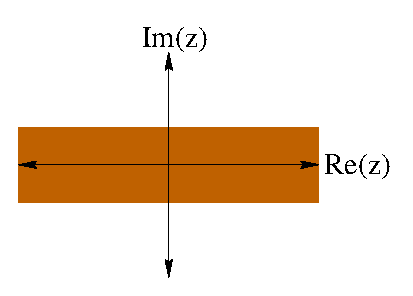
\includegraphics[width=0.25\textwidth]{ode/fourier_transform/fig_dom_conv}
    \end{center}
    \caption{The domain of convergence.}
    \label{fig_dom_conv}
  \end{figure}




  Now We do the integration.
  \begin{align*} 
    \mathcal{F}\left[ \e^{-a |x|} \right]
    &= \frac{1}{2\pi} \int_{-\infty}^0 \e^{( a - \imath \omega ) x}\,\dd x + 
    \frac{1}{2\pi} \int_0^\infty \e^{-(a + \imath \omega) x}\,\dd x 
    \\
    &= \frac{1}{2\pi} \left[ \frac{\e^{(a - \imath \omega)x}}{a - \imath \omega} \right]_{-\infty}^0 + 
    \frac{1}{2\pi} \left[ -\frac{\e^{-(a + \imath \omega) x}}{a + \imath \omega} \right]_0^\infty 
    \\
    &= \frac{1}{2\pi} \left( \frac{1}{a - \imath \omega} + \frac{1}{a + \imath \omega} \right) 
    \\
    &= \frac{1}{\pi} \frac{a}{\pi (\omega^2 + a^2)}, \quad \mathrm{for}\ |\Im(\omega)| < a
  \end{align*}
  We can extend the domain of the Fourier transform with analytic continuation.
  \[ 
  \mathcal{F}\left[\e^{-a |x|}\right] = 
  \frac{a}{\pi (\omega^2 + a^2)}, \quad \mathrm{for}\ \omega \neq \pm \imath a
  \]
\end{Example}













\begin{Example}
  Consider the Fourier transform of $f(x) = \frac{1}{x - \imath \alpha}$, 
  $\alpha > 0$.
  \[ 
  \mathcal{F}\left[\frac{1}{x - \imath \alpha} \right] 
  = \frac{1}{2\pi} \int_{-\infty}^\infty \frac{1}{x - \imath \alpha} \e^{-\imath \omega x}\,\dd x 
  \]
  The integral converges for $\Im(\omega) = 0$.  We will evaluate the integral
  for positive and negative real values of $\omega$.

  For $\omega > 0$, we will close the path of integration in the lower 
  half-plane.  Let $C_R$ be the contour from $x = R$ to $x = -R$ following a 
  semicircular path in the lower half-plane.  The integral along $C_R$ vanishes
  as $R \to \infty$ by Jordan's Lemma.
  \[ 
  \int_{C_R} \frac{1}{x - \imath \alpha} \e^{-\imath \omega x}\,\dd x \to 0 \quad 
  \mathrm{as}\ R \to \infty.
  \]
  Since the integrand is analytic in the lower half-plane the integral 
  vanishes.
  \[ 
  \mathcal{F}\left[\frac{1}{x - \imath \alpha} \right] = 0
  \]

  For $\omega < 0$, we will close the path of integration in the upper
  half-plane.  Let $C_R$ denote the semicircular contour from $x=R$ to $x=-R$
  in the upper half-plane.  The integral along $C_R$ vanishes as $R$ goes to
  infinity by Jordan's Lemma.  We evaluate the Fourier transform integral 
  with the Residue Theorem.
  \begin{align*}
    \mathcal{F}\left[\frac{1}{x - \imath \alpha} \right]
    &= \frac{1}{2\pi} 2\pi i\, \Res \left( \frac{\e^{-\imath \omega x}}{x-i\alpha}, i\alpha \right) 
    \\
    &= \imath \e^{\alpha \omega}
  \end{align*}

  We combine the results for positive and negative values of $\omega$.
  \[ 
  \mathcal{F}\left[\frac{1}{x - \imath \alpha} \right] = 
  \begin{cases}
    0 \quad &\mathrm{for}\ \omega > 0, \\
    \imath \e^{\alpha \omega} \quad &\mathrm{for}\ \omega < 0
  \end{cases}
  \]
\end{Example}




























%%---------------------------------------------------------------------------
\subsection{Cauchy Principal Value and Integrals that are Not Absolutely 
  Convergent.}
\index{principal value}
\index{Cauchy principal value}


That the integral of $f(x)$ is absolutely convergent is a sufficient but
not a necessary
condition that the Fourier transform of $f(x)$ exists.  The integral
$\int_{-\infty}^\infty f(x) \e^{-\imath \omega x}\,\dd x$ may converge even if $\int_{-\infty}^\infty |f(x)|\,\dd x$
does not.  Furthermore, if the Fourier transform integral diverges, 
its principal value may exist.  We will say that the Fourier transform 
of $f(x)$ exists if the principal value of the integral exists.
\[ 
\mathcal{F}[f(x)] = \pv \int_{-\infty}^\infty f(x) \e^{-\imath \omega x}\,\dd x
\]







\begin{Example}
  \label{ex_int_sin}
  Consider the Fourier transform of $f(x) = 1/x$.
  \[ 
  \hat{f}(\omega) = \frac{1}{2\pi} \pv \int_{-\infty}^\infty \frac{1}{x} \e^{-\imath \omega x}\,\dd x
  \]
  If $\omega > 0$, we can close the contour in the lower half-plane.
  The integral along the semi-circle vanishes due to Jordan's Lemma.
  \[ 
  \lim_{R \to \infty} \int_{C_R} \frac{1}{x} \e^{-\imath \omega x}\,\dd x = 0
  \]
  We can evaluate the Fourier transform with the Residue Theorem.
  \begin{gather*}
    \hat{f}(\omega) = \frac{1}{2\pi} \left(\frac{-1}{2}\right) (2 \pi i) \Res
    \left( \frac{1}{x} \e^{-\imath \omega x}, 0 \right) 
    \\
    \hat{f}(\omega) = -\frac{\imath}{2}, \quad \mathrm{for}\ \omega > 0.
  \end{gather*}

  The factor of $-1/2$ in the above derivation arises because the path of
  integration is in the negative, (clockwise), direction and the path
  of integration crosses through the first order pole at $x = 0$.
  The path of integration is shown in Figure~\ref{fig_one_half}.


  \begin{figure}[h!]
    \begin{center}
      \includegraphics[width=0.3\textwidth]{ode/fourier_transform/fig_one_half}
    \end{center}
    \caption{The path of integration.}
    \label{fig_one_half}
  \end{figure}



  If $\omega < 0$, we can close the contour in the upper half plane to 
  obtain
  \[
  \hat{f}(\omega) = \frac{\imath}{2}, \quad \mathrm{for}\ \omega < 0.
  \]
  For $\omega = 0$ the integral vanishes because
  $\frac{1}{x}$ is an odd function.
  \[
  \hat{f}(0) = \frac{1}{2\pi} = \pv \int_{-\infty}^\infty \frac{1}{x} \,\dd x = 0
  \]
  We collect the results in one formula.
  \[
  \boxed{
    \hat{f}(\omega) = - \frac{\imath}{2} \sign(\omega)
    }
  \]







  We write the integrand for $\omega > 0$ as the sum of an odd and 
  and even function.
  \begin{gather*}
    \frac{1}{2\pi} \pv \int_{-\infty}^\infty \frac{1}{x} \e^{-\imath \omega x}\,\dd x = - \frac{\imath}{2} 
    \\
    \pv \int_{-\infty}^\infty \frac{1}{x} \cos(\omega x)\,\dd x +
    \pv \int_{-\infty}^\infty \frac{- \imath}{x} \sin(\omega x)\,\dd x = -\imath \pi
    \\
    \intertext{The principal value of the integral of any odd function is zero.}
    \pv \int_{-\infty}^\infty \frac{1}{x} \sin(\omega x)\,\dd x = \pi 
    \\
    \intertext{If the principal value of the integral of an even function exists,
      then the integral converges.}
    \int_{-\infty}^\infty \frac{1}{x} \sin(\omega x)\,\dd x = \pi 
    \\
    \boxed{ 
      \int_0^\infty \frac{1}{x} \sin(\omega x)\,\dd x = \frac{\pi}{2}
      }
  \end{gather*}
  Thus we have evaluated an integral that we used in deriving the Fourier
  transform.
\end{Example}














%%---------------------------------------------------------------------------
\subsection{Analytic Continuation}
\index{Analytic continuation!Fourier integrals}









Consider the Fourier transform of $f(x) = 1$.  The Fourier integral is
not convergent, and its principal value does not exist.  Thus we will
have to be a little creative in order to define the Fourier transform.
Define the two functions
\[ 
f_+(x) = \begin{cases} 
  1 &\mathrm{for}\ x > 0 
  \\ 
  1/2 &\mathrm{for}\ x = 0 
  \\ 
  0 &\mathrm{for}\ x < 0 
\end{cases}, \qquad
f_-(x) = \begin{cases} 
  0 &\mathrm{for}\ x > 0 
  \\ 
  1/2 &\mathrm{for}\ x = 0 
  \\ 
  1 &\mathrm{for}\ x < 0 
\end{cases}. 
\]
Note that $1 = f_-(x) + f_+(x)$.

The Fourier transform of $f_+(x)$ converges for $\Im(\omega) < 0$.
\begin{align*}
  \mathcal{F}[f_+(x)]
  &= \frac{1}{2\pi} \int_0^\infty \e^{-\imath \omega x}\,\dd x 
  \\
  &= \frac{1}{2\pi} \int_0^\infty \e^{(-\imath \Re(\omega) + \Im(\omega))x} \,\dd x. 
  \\
  &= \frac{1}{2\pi} \left[ \frac{\e^{-\imath \omega x}}{-\imath \omega} \right]_0^\infty 
  \\
  &= -\frac{\imath}{2 \pi \omega} \quad \mathrm{for}\ \Im(\omega) < 0
\end{align*}
Using analytic continuation, we can define the Fourier transform of $f_+(x)$
for all $\omega$ except the point $\omega = 0$.
\[ 
\mathcal{F}[f_+(x)] = -\frac{\imath}{2\pi\omega}
\]


We follow the same procedure for $f_-(x)$.
The integral converges for $\Im(\omega) > 0$.
\begin{align*}
  \mathcal{F}[f_-(x)]
  &= \frac{1}{2\pi} \int_{-\infty}^0 \e^{-\imath \omega x}\,\dd x 
  \\
  &= \frac{1}{2\pi} \int_{-\infty}^0 \e^{(-\imath \Re(\omega) + \Im(\omega))x} \,\dd x
  \\
  &= \frac{1}{2\pi} \left[ \frac{\e^{-\imath \omega x}}{-\imath \omega} \right]_{-\infty}^0 
  \\
  &= \frac{\imath}{2 \pi \omega}.
\end{align*}
Using analytic continuation we can define the transform for all nonzero 
$\omega$.
\[ 
\mathcal{F}[f_-(x)] = \frac{\imath}{2 \pi \omega}
\]

Now we are prepared to define the Fourier transform of $f(x) = 1$.
\begin{align*}
  \mathcal{F}[1]
  &= \mathcal{F}[f_-(x)] + \mathcal{F}[f_+(x)] 
  \\
  &= -\frac{\imath}{2\pi\omega} + \frac{\imath}{2 \pi \omega} 
  \\
  &= 0 , \quad \mathrm{for}\ \omega \neq 0
\end{align*}
When $\omega = 0$ the integral diverges.  When we consider the 
closure relation for the Fourier transform we will see that
\[ 
\boxed{ 
  \mathcal{F}[1] = \delta(\omega). 
  } 
\]








%%===========================================================================
\section{Properties of the Fourier Transform}


In this section we will explore various properties of the Fourier Transform.
I would like to avoid stating assumptions on various functions at the beginning
of each subsection.  Unless otherwise indicated, 
assume that the integrals converge.




%%---------------------------------------------------------------------------
\subsection{Closure Relation.}
\index{Fourier transform!closure relation}
\index{closure relation!and Fourier transform}




Recall the closure relation for an orthonormal set of functions
$\{\phi_1, \phi_2, \ldots \}$,
\[ 
\sum_{n = 1}^\infty \phi_n(x) \overline{\phi_n(\xi)} \sim \delta(x-\xi).
\]
There is a similar closure relation for Fourier integrals.  We compute 
the Fourier transform of $\delta(x-\xi)$.
\begin{align*}
  \mathcal{F}[\delta(x-\xi)] 
  &= \frac{1}{2\pi} \int_{-\infty}^\infty \delta(x-\xi) \e^{-\imath \omega x}\,\dd x 
  \\
  &= \frac{1}{2\pi} \e^{-\imath \omega \xi}
\end{align*}
Next we take the inverse Fourier transform.
\begin{gather*}
  \delta(x-\xi) \sim \int_{-\infty}^\infty \frac{1}{2 \pi} \e^{-\imath \omega \xi} \e^{\imath \omega x}\,\dd \omega
  \\
  \boxed{ 
    \delta(x-\xi) \sim \frac{1}{2 \pi} \int_{-\infty}^\infty \e^{\imath \omega (x-\xi)}\,\dd \omega. 
    }
\end{gather*}
Note that the integral is divergent, but it would be impossible to
represent $\delta(x-\xi)$ with a convergent integral.








%%---------------------------------------------------------------------------
\subsection{Fourier Transform of a Derivative.}
\index{Fourier transform!of a derivative}



Consider the Fourier transform of $y'(x)$.
\begin{align*}
  \mathcal{F}[y'(x)]
  &= \frac{1}{2\pi} \int_{-\infty}^\infty y'(x) \e^{-\imath \omega x}\,\dd x 
  \\
  &= \left[\frac{1}{2\pi} y(x) \e^{-\imath \omega x} \right]_{-\infty}^\infty
  - \frac{1}{2\pi} \int_{-\infty}^\infty (-\imath \omega) y(x) \e^{-\imath \omega x}\,\dd x 
  \\
  &= \imath \omega \frac{1}{2\pi} \int_{-\infty}^\infty y(x) \e^{-\imath \omega x}\,\dd x 
  \\
  &= \imath \omega \mathcal{F}[y(x)]
\end{align*}
Next consider $y''(x)$.
\begin{align*}
  \mathcal{F}[y''(x)]
  &= \mathcal{F}\left[ \frac{\dd}{\dd x}(y'(x)) \right] 
  \\
  &= \imath \omega \mathcal{F}[y'(x)] 
  \\
  &= (\imath \omega)^2 \mathcal{F}[y(x)] 
  \\
  &= - \omega^2 \mathcal{F}[y(x)]
\end{align*}
In general,
\[ 
\boxed{ 
  \mathcal{F}\left[y^{(n)}(x)\right] = (\imath \omega)^n \mathcal{F}[y(x)]. 
  } 
\]







\begin{Example}
  The Dirac delta function can be expressed as the derivative of the 
  Heaviside function.
  \[ 
  H(x-c) = 
  \begin{cases}
    0 \quad &\mathrm{for}\ x < c, \\
    1 \quad &\mathrm{for}\ x > c
  \end{cases}
  \]
  Thus we can express the Fourier transform of $H(x-c)$ in terms of the Fourier
  transform of the delta function.
  \begin{gather*}
    \mathcal{F}[\delta(x-c)] = \imath \omega \mathcal{F}[H(x-c)] 
    \\
    \frac{1}{2\pi} \int_{-\infty}^\infty \delta(x-c) \e^{-\imath \omega x}\,\dd x = \imath \omega \mathcal{F}[H(x-c)] 
    \\
    \frac{1}{2\pi} \e^{-\imath c \omega} = \imath \omega \mathcal{F}[H(x-c)]
  \end{gather*}
  \[ 
  \boxed{ 
    \mathcal{F}[H(x-c)] = \frac{1}{2\pi \imath \omega} \e^{-\imath c \omega}
    } 
  \]
\end{Example}



















%%---------------------------------------------------------------------------
\subsection{Fourier Convolution Theorem.}
\index{convolution theorem!and Fourier transform}
\index{Fourier transform!convolution theorem}
\index{Fourier convolution theorem}



Consider the Fourier transform of a product of two functions.
\begin{align*}
  \mathcal{F}[f(x)g(x)]
  &= \frac{1}{2\pi} \int_{-\infty}^\infty f(x) g(x) \e^{-\imath \omega x}\,\dd x 
  \\
  &= \frac{1}{2\pi} \int_{-\infty}^\infty \left( \int_{-\infty}^\infty \hat{f}(\eta) \e^{\imath \eta x}\,\dd \eta
  \right) g(x) \e^{-\imath \omega x}\,\dd x 
  \\
  &= \frac{1}{2\pi} \int_{-\infty}^\infty \left( \int_{-\infty}^\infty \hat{f}(\eta) g(x) 
    \e^{\imath (\eta - \omega)x} \,\dd x \right) \,\dd \eta 
  \\
  &= \int_{-\infty}^\infty \hat{f}(\eta) \left( \frac{1}{2\pi} \int_{-\infty}^\infty g(x) \e^{-\imath 
      (\omega - \eta) x}\,\dd x \right)\,\dd \eta 
  \\
  &= \int_{-\infty}^\infty \hat{f}(\eta) G(\omega - \eta)\,\dd \eta
\end{align*}
The convolution of two functions is defined
\[ 
f * g(x) = \int_{-\infty}^\infty f(\xi) g(x-\xi)\,\dd \xi.
\]
Thus
\[ 
\boxed{ 
  \mathcal{F}[f(x)g(x)] = \hat{f} * \hat{g}(\omega) 
  = \int_{-\infty}^\infty \hat{f}(\eta) \hat{g}(\omega - \eta)\,\dd \eta.
  } 
\]






Now consider the inverse Fourier Transform of a product of two functions.
\begin{align*}
  \mathcal{F}^{-1}[\hat{f}(\omega)\hat{g}(\omega)]
  &= \int_{-\infty}^\infty \hat{f}(\omega)\hat{g}(\omega) \e^{\imath \omega x}\,\dd \omega 
  \\
  &= \int_{-\infty}^\infty \left(\frac{1}{2\pi} \int_{-\infty}^\infty f(\xi) \e^{-\imath \omega \xi}\,\dd \xi
  \right) \hat{g}(\omega) \e^{\imath \omega x}\,\dd \omega 
  \\
  &= \frac{1}{2\pi} \int_{-\infty}^\infty \left( \int_{-\infty}^\infty f(\xi) \hat{g}(\omega) 
    \e^{\imath \omega(x-\xi)} \,\dd \omega \right) \,\dd \xi 
  \\
  &= \frac{1}{2\pi} \int_{-\infty}^\infty f(\xi) \left( 
    \int_{-\infty}^\infty \hat{g}(\omega) \e^{\imath \omega (x-\xi)}\,\dd \omega \right) \,\dd \xi 
  \\
  &= \frac{1}{2\pi} \int_{-\infty}^\infty f(\xi) g(x-\xi)\,\dd \xi 
\end{align*}
Thus
\begin{gather*} 
  \boxed{ 
    \mathcal{F}^{-1}[\hat{f}(\omega)\hat{g}(\omega)] 
    = \frac{1}{2\pi} f * g (x)
    = \frac{1}{2\pi} \int_{-\infty}^\infty f(\xi) g(x-\xi)\,\dd \xi,
    } 
  \\
  \boxed{ 
    \mathcal{F}[f * g (x)] = 2 \pi \hat{f}(\omega)\hat{g}(\omega).
    } 
\end{gather*}

These relations are known as the Fourier convolution theorem.





\begin{Example}
  Using the convolution theorem and the table of Fourier transform pairs in the
  appendix, we can find the Fourier transform of
  \[ 
  f(x) = \frac{1}{x^4 + 5 x^2 + 4}. 
  \]
  We factor the fraction.
  \[ 
  f(x) = \frac{1}{(x^2+1)(x^2+4)}
  \]
  From the table, we know that
  \[ 
  \mathcal{F} \left[ \frac{2c}{x^2+c^2} \right] = \e^{-c |\omega|} \quad \mathrm{for}\ c > 0. 
  \]
  We apply the convolution theorem.
  \begin{align*}
    \mathcal{F}[f(x)]
    &= \mathcal{F} \left[ \frac{1}{8} \frac{2}{x^2+1} \frac{4}{x^2+4} \right] 
    \\
    &= \frac{1}{8} \left( \int_{-\infty}^\infty \e^{-|\eta|} \e^{-2|\omega - \eta|}\,\dd \eta \right) 
    \\
    &= \frac{1}{8} \left( \int_{-\infty}^0 \e^\eta \e^{-2|\omega - \eta|}\,\dd \eta
      + \int_0^\infty \e^{-\eta} \e^{-2|\omega - \eta|}\,\dd \eta \right)
  \end{align*}
  First consider the case $\omega > 0$.
  \begin{align*}
    \mathcal{F}[f(x)]
    &= \frac{1}{8} \left( \int_{-\infty}^0 \e^{-2\omega + 3\eta}\,\dd \eta
      + \int_0^\omega \e^{-2\omega + \eta}\,\dd \eta
      + \int_\omega^\infty \e^{2\omega - 3 \eta}\,\dd \eta \right) 
    \\
    &= \frac{1}{8} \left( \frac{1}{3} \e^{-2\omega} + \e^{-\omega}
      - \e^{-2\omega} + \frac{1}{3} \e^{-\omega} \right) 
    \\
    &= \frac{1}{6} \e^{-\omega} - \frac{1}{12} \e^{-2\omega}
  \end{align*}
  Now consider the case $\omega < 0$.
  \begin{align*}
    \mathcal{F}[f(x)]
    &= \frac{1}{8} \left( \int_{-\infty}^\omega \e^{-2\omega+3\eta}\,\dd \eta
      + \int_\omega^0 \e^{2\omega - \eta}\,\dd \eta
      + \int_0^\infty \e^{2\omega-3\eta}\,\dd \eta \right) 
    \\
    &= \frac{1}{8} \left( \frac{1}{3} \e^\omega - \e^{2\omega}
      + \e^\omega + \frac{1}{3} \e^{2\omega} \right) \\
    &= \frac{1}{6} \e^\omega - \frac{1}{12} \e^{2\omega} 
  \end{align*}
  We collect the result for positive and negative $\omega$.
  \[ 
  \boxed{ 
    \mathcal{F}[f(x)] = \frac{1}{6} \e^{-|\omega|} - \frac{1}{12} \e^{-2|\omega|} 
    } 
  \]

  A better way to find the Fourier transform of 
  \[
  f(x) = \frac{1}{x^4 + 5 x^2 + 4}
  \]
  is to first expand the function in partial fractions.
  \[
  f(x) = \frac{1/3}{x^2 + 1} - \frac{1/3}{x^2 + 4}
  \]
  \begin{align*}
    \mathcal{F}[f(x)]
    &= \frac{1}{6} \mathcal{F} \left[ \frac{2}{x^2 + 1} \right]
    - \frac{1}{12} \mathcal{F} \left[ \frac{4}{x^2+4} \right] 
    \\
    &= \frac{1}{6} \e^{-|\omega|} - \frac{1}{12} \e^{-2|\omega|}
  \end{align*}
\end{Example}






















%%---------------------------------------------------------------------------
\subsection{Parseval's Theorem.}
\index{Parseval's theorem!for Fourier transform}
\index{Fourier transform!Parseval's theorem}




Recall Parseval's theorem for Fourier series.  If $f(x)$ is a complex
valued function with the Fourier series $\sum_{n = - \infty}^\infty c_n \e^{\imath n x}$ then
\[ 
2 \pi \sum_{n = - \infty}^\infty |c_n|^2 = \int_{-\pi}^\pi |f(x)|^2\,\dd x. 
\]
Analogous to this result is Parseval's theorem for Fourier transforms.

Let $f(x)$ be a complex valued function that is both absolutely integrable
and square integrable.
\[ 
\int_{-\infty}^\infty |f(x)|\,\dd x < \infty \quad \mathrm{and} \quad
\int_{-\infty}^\infty |f(x)|^2 \,\dd x < \infty
\]

The Fourier transform of $\overline{f(-x)}$ is $\overline{\hat{f}(\omega)}$.
\begin{align*}
  \mathcal{F}\left[\overline{f(-x)}\right]
  &= \frac{1}{2\pi} \int_{-\infty}^\infty \overline{f(-x)} \e^{-\imath \omega x} \,\dd x 
  \\
  &= - \frac{1}{2\pi} \int_\infty^{-\infty} \overline{f(x)} \e^{\imath \omega x} \,\dd x 
  \\
  &= \frac{1}{2\pi} \int_{-\infty}^\infty \overline{f(x) \e^{-\imath \omega x}} \,\dd x 
  \\
  &= \overline{\hat{f}(\omega)}
\end{align*}

We apply the convolution theorem.
\begin{gather*}
  \mathcal{F}^{-1} [2\pi \hat{f}(\omega) \overline{\hat{f}(\omega)}] = 
  \int_{-\infty}^\infty f(\xi) \overline{f(-(x-\xi))}\,\dd \xi 
  \\
  \int_{-\infty}^\infty 2 \pi \hat{f}(\omega) \overline{\hat{f}(\omega)} \e^{\imath \omega x}\,\dd \omega
  = \int_{-\infty}^\infty f(\xi) \overline{f(\xi-x)}\,\dd \xi
  \\
  \intertext{We set $x=0$.}
  2 \pi \int_{-\infty}^\infty \hat{f}(\omega) \overline{\hat{f}(\omega)} \,\dd \omega
  = \int_{-\infty}^\infty f(\xi) \overline{f(\xi)}\,\dd \xi 
  \\
  \boxed{ 
    2 \pi \int_{-\infty}^\infty |\hat{f}(\omega)|^2\,\dd \omega = \int_{-\infty}^\infty |f(x)|^2\,\dd x
    }
\end{gather*}
This is known as \textbf{Parseval's theorem}.







%%---------------------------------------------------------------------------
\subsection{Shift Property.}
\index{Fourier transform!shift property}




The Fourier transform of $f(x+c)$ is
\begin{align*}
  \mathcal{F}[f(x+c)]
  &= \frac{1}{2\pi} \int_{-\infty}^\infty f(x+c) \e^{-\imath \omega x}\,\dd x 
  \\
  &= \frac{1}{2\pi} \int_{-\infty}^\infty f(x) \e^{-\imath \omega (x-c)}\,\dd x 
\end{align*}
\[ 
\boxed{ 
  \mathcal{F}[f(x+c)] = \e^{\imath \omega c} \hat{f}(\omega)
  } 
\]

The inverse Fourier transform of $\hat{f}(\omega+c)$ is
\begin{align*}
  \mathcal{F}^{-1}[\hat{f}(\omega+c)]
  &= \int_{-\infty}^\infty \hat{f}(\omega+c) \e^{\imath \omega x}\,\dd \omega 
  \\
  &= \int_{-\infty}^\infty \hat{f}(\omega) \e^{\imath (\omega - c) x}\,\dd \omega 
\end{align*}
\[ 
\boxed{ 
  \mathcal{F}^{-1}[\hat{f}(\omega+c)] = \e^{-\imath c x} f(x)
  } 
\]







%%---------------------------------------------------------------------------
\subsection{Fourier Transform of x f(x).}



The Fourier transform of $x f(x)$ is
\begin{align*}
  \mathcal{F}[x f(x)]
  &= \frac{1}{2\pi} \int_{-\infty}^\infty x f(x) \e^{-\imath \omega x}\,\dd x 
  \\
  &= \frac{1}{2\pi} \int_{-\infty}^\infty \imath f(x) \frac{\partial}{\partial \omega}(\e^{-\imath \omega x}) \,\dd x 
  \\
  &= \imath \frac{\partial}{\partial \omega} \left( \frac{1}{2\pi} \int_{-\infty}^\infty f(x) \e^{-\imath \omega x}\,\dd x \right) 
\end{align*}
\[ 
\boxed{ 
  \mathcal{F}[x f(x)] = \imath \frac{\partial \hat{f}}{\partial \omega}.
  } 
\]

Similarly, you can show that
\[ 
\boxed{
  \mathcal{F}[x^n f(x)] = (i)^n \frac{\partial^n \hat{f}}{\partial \omega^n}.
  } 
\]














%%===========================================================================
\section{Solving Differential Equations with the Fourier Transform}


The Fourier transform is useful in solving some differential equations on
the domain $(-\infty \ldots \infty)$ with homogeneous boundary conditions at infinity.  
We take the Fourier transform of the differential equation 
$L[y] = f$ and solve for $\hat{y}$.  We take the inverse transform to 
determine the solution $y$.  Note that this process is only applicable if
the Fourier transform of $y$ exists.  Hence the requirement for homogeneous
boundary conditions at infinity.  

We will use the table of Fourier transforms in the appendix 
in solving the examples in this section.











\begin{Example}
  Consider the problem
  \[ 
  y'' - y = \e^{-\alpha |x|}, \qquad y(\pm \infty) = 0, \qquad \alpha > 0, \alpha \neq 1.
  \]
  We take the Fourier transform of this equation.
  \[
  -\omega^2 \hat{y}(\omega) - \hat{y}(\omega) = \frac{\alpha / \pi}{\omega^2 + \alpha^2}
  \]
  We take the inverse Fourier transform to determine the solution.
  \begin{align*}
    \hat{y}(\omega)
    &= \frac{-\alpha/ \pi}{(\omega^2+\alpha^2)(\omega^2+1)} 
    \\
    &= \frac{-\alpha}{\pi} \frac{1}{\alpha^2-1} \left(
      \frac{1}{\omega^2 + 1} - \frac{1}{\omega^2 + \alpha^2} \right) 
    \\
    &= \frac{1}{\alpha^2 - 1} \left( \frac{\alpha / \pi}{\omega^2 + \alpha^2}
      - \alpha \frac{1/\pi}{\omega^2 + 1} \right)
  \end{align*}
  \[ 
  \boxed{ 
    y(x) = \frac{\e^{-\alpha |x|} - \alpha \e^{-|x|}}{\alpha^2-1}
    }
  \]
\end{Example}













\begin{Example}
  Consider the Green function problem
  \[ 
  G'' - G = \delta(x-\xi), \qquad y(\pm \infty) = 0.
  \]
  We take the Fourier transform of this equation.
  \begin{gather*}
    -\omega^2 \hat{G} - \hat{G} = \mathcal{F}[ \delta(x - \xi) ]
    \\
    \hat{G} = - \frac{1}{\omega^2 + 1} \mathcal{F}[ \delta(x - \xi) ]
    \\
    \intertext{We use the Table of Fourier transforms.}
    \hat{G} = - \pi \mathcal{F}\left[ \e^{-|x|} \right] \mathcal{F}[ \delta(x - \xi) ]
    \\
    \intertext{We use the convolution theorem to do the inversion.}
    G = - \pi \frac{1}{2 \pi} \int_{-\infty}^\infty \e^{-|x - \eta|} \delta(\eta - \xi) \,\dd \eta
    \\
    G(x|\xi) = - \frac{1}{2} \e^{|x - \xi|}
  \end{gather*}
  The inhomogeneous differential equation
  \[ 
  y'' - y = f(x), \qquad y(\pm \infty) = 0,
  \]
  has the solution
  \[ 
  \boxed{ 
    y = - \frac{1}{2} \int_{-\infty}^\infty f(\xi) \e^{-|x-\xi|}\,\dd \xi. 
    } 
  \]
\end{Example}







When solving the differential equation $L[y] = f$ with the Fourier transform, 
it is quite common to use the convolution theorem.  With this approach we 
have no need to compute the Fourier transform of the right side.  We merely
\textit{denote} it as $\mathcal{F}[f]$ until we use $f$ in the convolution
integral.














%%===========================================================================
\section{The Fourier Cosine and Sine Transform}






%%---------------------------------------------------------------------------
\subsection{The Fourier Cosine Transform}
\index{Fourier cosine transform}





Suppose $f(x)$ is an even function.  
In this case the Fourier transform of $f(x)$ coincides with the 
\textit{Fourier cosine transform} of $f(x)$.
\begin{align*}
  \mathcal{F}[f(x)]
  &= \frac{1}{2\pi} \int_{-\infty}^\infty f(x) \e^{-\imath \omega x}\,\dd x 
  \\
  &= \frac{1}{2\pi} \int_{-\infty}^\infty f(x) (\cos(\omega x) - \imath \sin(\omega x)) \,\dd x 
  \\
  &= \frac{1}{2\pi} \int_{-\infty}^\infty f(x) \cos(\omega x)\,\dd x 
  \\
  &= \frac{1}{\pi} \int_0^\infty f(x) \cos(\omega x)\,\dd x
\end{align*}
The Fourier cosine transform is defined:
\[ 
\mathcal{F}_c[f(x)] = \hat{f}_c(\omega) = \frac{1}{\pi} \int_0^\infty f(x) \cos(\omega x)\,\dd x.
\]

Note that $\hat{f}_c(\omega)$ is an even function.  The inverse Fourier cosine 
transform is
\begin{align*}
  \mathcal{F}_c^{-1}[\hat{f}_c(\omega)]
  &= \int_{-\infty}^\infty \hat{f}_c(\omega) \e^{\imath \omega x}\,\dd \omega 
  \\
  &= \int_{-\infty}^\infty \hat{f}_c(\omega) (\cos(\omega x) + \imath \sin(\omega x))\,\dd \omega 
  \\
  &= \int_{-\infty}^\infty \hat{f}_c(\omega) \cos(\omega x)\,\dd \omega 
  \\
  &= 2 \int_0^\infty \hat{f}_c(\omega) \cos(\omega x)\,\dd \omega.
\end{align*}

Thus we have the Fourier cosine transform pair
\[ 
f(x) = \mathcal{F}_c^{-1}[\hat{f}_c(\omega)] = 2 \int_0^\infty \hat{f}_c(\omega) \cos(\omega x)\,\dd \omega, 
\qquad
\hat{f}_c(\omega) = \mathcal{F}_c[f(x)]=\frac{1}{\pi} \int_0^\infty f(x) \cos(\omega x)\,\dd x.
\]











%%---------------------------------------------------------------------------
\subsection{The Fourier Sine Transform}
\index{Fourier sine transform}


Suppose $f(x)$ is an odd function.
In this case the Fourier transform of $f(x)$ coincides with the 
\textit{Fourier sine transform} of $f(x)$.
\begin{align*}
  \mathcal{F}[f(x)] 
  &= \frac{1}{2\pi} \int_{-\infty}^\infty f(x) \e^{-\imath \omega x}\,\dd x 
  \\
  &= \frac{1}{2\pi} \int_{-\infty}^\infty f(x) (\cos(\omega x) - \imath \sin(\omega x)) \,\dd x 
  \\
  &= - \frac{\imath}{\pi} \int_0^\infty f(x) \sin(\omega x)\,\dd x
\end{align*}
Note that $\hat{f}(\omega) = \mathcal{F}[f(x)]$ is an odd function of $\omega$.  
The inverse Fourier transform of $\hat{f}(\omega)$ is
\begin{align*}
  \mathcal{F}^{-1}[\hat{f}(\omega)]
  &= \int_{-\infty}^\infty \hat{f}(\omega) \e^{\imath \omega x}\,\dd \omega 
  \\
  &= 2 \imath \int_0^\infty \hat{f}(\omega) \sin(\omega x)\,\dd \omega.
\end{align*}

Thus we have that 
\begin{align*}
  f(x)    
  &= 2 \imath \int_0^\infty \left( - \frac{\imath}{\pi} \int_0^\infty f(x) \sin(\omega x)
    \,\dd x \right) \sin(\omega x)\,\dd \omega 
  \\
  &= 2 \int_0^\infty \left( \frac{1}{\pi} \int_0^\infty f(x) \sin(\omega x)\,\dd x
  \right) \sin(\omega x) \,\dd \omega.
\end{align*}
This gives us the Fourier sine transform pair
\[ 
f(x) = \mathcal{F}_s^{-1}[\hat{f}_s(\omega)] = 2 \int_0^\infty \hat{f}_s(\omega) \sin(\omega x)\,\dd \omega, 
\qquad 
\hat{f}_s(\omega) = \mathcal{F}_s[f(x)] = \frac{1}{\pi} \int_0^\infty f(x)\sin(\omega x)\,\dd x.
\]







\begin{Result}
  The Fourier cosine transform pair is defined:
  \begin{align*}
    f(x) &= \mathcal{F}_c^{-1}[\hat{f}_c(\omega)] = 2 \int_0^\infty \hat{f}_c(\omega) \cos(\omega x)\,\dd \omega 
    \\
    \hat{f}_c(\omega) &= \mathcal{F}_c[f(x)] = \frac{1}{\pi} \int_0^\infty f(x) \cos(\omega x)\,\dd x
  \end{align*}
  The Fourier sine transform pair is defined:
  \begin{align*}
    f(x) &= \mathcal{F}_s^{-1}[\hat{f}_s(\omega)] = 2 \int_0^\infty \hat{f}_s(\omega) \sin(\omega x)\,\dd \omega 
    \\
    \hat{f}_s(\omega) &= \mathcal{F}_s[f(x)] = \frac{1}{\pi} \int_0^\infty f(x)\sin(\omega x)\,\dd x
  \end{align*}
\end{Result}










%%===========================================================================
\section{Properties of the Fourier Cosine and Sine Transform}






%%--------------------------------------------------------------------------
\subsection{Transforms of Derivatives}
\index{Fourier sine transform!of derivatives}
\index{Fourier cosine transform!of derivatives}





\paragraph{Cosine Transform.}
Using integration by parts we can find the Fourier cosine transform of 
derivatives.  Let $y$ be a function for which the Fourier cosine transform
of $y$ and its first and second derivatives exists.  Further assume that
$y$ and $y'$ vanish at infinity.
We calculate the transforms of the first and second derivatives.
\begin{align*}
  \mathcal{F}_c[y'] &= \frac{1}{\pi} \int_0^\infty y' \cos(\omega x)\,\dd x 
  \\
  &= \frac{1}{\pi} \big[y \cos(\omega x)\big]_0^\infty 
  + \frac{\omega}{\pi} \int_0^\infty y \sin(\omega x)\,\dd x 
  \\
  &= \omega \hat{y}_c(\omega) - \frac{1}{\pi} y(0) 
  \\
  \mathcal{F}_c[y''] &= \frac{1}{\pi} \int_0^\infty y'' \cos(\omega x)\,\dd x 
  \\
  &= \frac{1}{\pi} \big[y' \cos(\omega x)\big]_0^\infty 
  + \frac{\omega}{\pi} \int_0^\infty y' \sin(\omega x)\,\dd x 
  \\
  &= - \frac{1}{\pi} y'(0) + \frac{\omega}{\pi}\big[y \sin(\omega x)
  \big]_0^\infty - \frac{\omega^2}{\pi} \int_0^\infty y \cos(\omega x) \,\dd x 
  \\
  &= - \omega^2 \hat{f}_c(\omega) - \frac{1}{\pi} y'(0)
\end{align*}


\paragraph{Sine Transform.}
You can show, (see Exercise~\ref{exercise ode ft fst y' y''}), that the Fourier
sine transform of the first and second derivatives are
\begin{align*}
  \mathcal{F}_s[y'] &= - \omega \hat{f}_c(\omega) 
  \\
  \mathcal{F}_s[y''] &= - \omega^2 \hat{y}_c(\omega) + \frac{\omega}{\pi} y(0).
\end{align*}












%%--------------------------------------------------------------------------
\subsection{Convolution Theorems}



\paragraph{Cosine Transform of a Product.}
Consider the Fourier cosine transform of a product of functions.
Let $f(x)$ and $g(x)$ be two functions defined for $x \geq 0$.
Let $\mathcal{F}_c[f(x)] = \hat{f}_c(\omega)$, and $\mathcal{F}_c[g(x)] = 
\hat{g}_c(\omega)$.
\begin{align*}
  \mathcal{F}_c[f(x)g(x)]
  &= \frac{1}{\pi} \int_0^\infty f(x) g(x) \cos(\omega x)\,\dd x 
  \\
  &= \frac{1}{\pi} \int_0^\infty \left( 2 \int_0^\infty \hat{f}_c(\eta) \cos(\eta x)\,\dd \eta \right) 
  g(x) \cos(\omega x)\,\dd x 
  \\
  &= \frac{2}{\pi} \int_0^\infty \int_0^\infty \hat{f}_c(\eta) g(x) \cos(\eta x) 
  \cos(\omega x)\,\dd x\,\dd \eta 
  \\
  \intertext{We use the identity $\cos a \cos b = \frac{1}{2}(\cos(a-b) 
    + \cos(a+b))$.}
  &= \frac{1}{\pi} \int_0^\infty \int_0^\infty \hat{f}_c(\eta) g(x) \big( \cos((\omega-\eta)x)
  + \cos((\omega + \eta) x) \big)\,\dd x \,\dd \eta 
  \\
  &= \int_0^\infty \hat{f}_c(\eta) \left[ \frac{1}{\pi} \int_0^\infty g(x) 
    \cos((\omega-\eta)x)\,\dd x + \frac{1}{\pi} \int_0^\infty g(x) 
    \cos((\omega+\eta)x)\,\dd x \right]\,\dd \eta 
  \\
  &= \int_0^\infty \hat{f}_c(\eta) \big(\hat{g}_c(\omega-\eta) 
  + \hat{g}_c(\omega+\eta) \big)\,\dd \eta 
  \\
  \intertext{$\hat{g}_c(\omega)$ is an even function.  If we have only defined
    $\hat{g}_c(\omega)$ for positive argument, then $\hat{g}_c(\omega) = 
    \hat{g}_c(|\omega|)$.}
  &= \int_0^\infty \hat{f}_c(\eta) \big(\hat{g}_c(|\omega-\eta|) + \hat{g}_c(\omega+\eta) \big)\,\dd \eta 
\end{align*}




\paragraph{Inverse Cosine Transform of a Product.}
Now consider the inverse Fourier cosine transform of a product of functions.
Let $\mathcal{F}_c[f(x)] = \hat{f}_c(\omega)$, and 
$\mathcal{F}_c[g(x)] = \hat{g}_c(\omega)$.
\begin{align*}
  \mathcal{F}_c^{-1}[\hat{f}_c(\omega) \hat{g}_c(\omega)]
  &= 2 \int_0^\infty \hat{f}_c(\omega) \hat{g}_c(\omega) \cos(\omega x)\,\dd \omega 
  \\
  &= 2 \int_0^\infty \left( \frac{1}{\pi} \int_0^\infty f(\xi) \cos(\omega \xi)\,\dd \xi
  \right) \hat{g}_c(\omega) \cos(\omega x)\,\dd \omega 
  \\
  &= \frac{2}{\pi} \int_0^\infty \int_0^\infty f(\xi) \hat{g}_c(\omega) \cos(\omega \xi) \cos(\omega x)\,\dd \omega \,\dd \xi 
  \\
  &= \frac{1}{\pi} \int_0^\infty \int_0^\infty f(\xi) \hat{g}_c(\omega) \big(\cos(\omega(x-\xi)) + \cos(\omega(x+\xi))
  \big)\,\dd \omega\,\dd \xi 
  \\
  &= \frac{1}{2\pi}\int_0^\infty f(\xi) \left( 2 \int_0^\infty \hat{g}_c(\omega) 
    \cos(\omega(x-\xi))\,\dd \omega + 2 \int_0^\infty \hat{g}_c(\omega)
    \cos(\omega(x+\xi))\,\dd \omega \right) \,\dd \xi 
  \\
  &= \frac{1}{2\pi}\int_0^\infty f(\xi) \big(g(|x-\xi|) + g(x+\xi)\big)\,\dd \xi
\end{align*}


\paragraph{Sine Transform of a Product.}
You can show, (see Exercise~\ref{exercise ode ft sine convolution}),
that the Fourier sine transform of a product of functions is
\[ 
\mathcal{F}_s[f(x)g(x)] = \int_0^\infty \hat{f}_s(\eta) \big(\hat{g}_c(|\omega-\eta|)
- \hat{g}_c(\omega+\eta) \big) \,\dd \eta.  
\]

\paragraph{Inverse Sine Transform of a Product.}
You can also show, (see 
Exercise~\ref{exercise ode ft inverse sine convolution}),
that the inverse Fourier sine transform of a product of functions is
\[ 
\mathcal{F}_s^{-1}[\hat{f}_s(\omega) \hat{g}_c(\omega)] 
= \frac{1}{2\pi} \int_0^\infty f(\xi) \big(g(|x-\xi|) - g(x+\xi) \big) \,\dd \xi.
\]


\begin{Result}
  The Fourier cosine and sine transform convolution theorems are
  \begin{gather*}
    \mathcal{F}_c[f(x) g(x)] = \int_0^\infty \hat{f}_c(\eta) \big[\hat{g}_c(|\omega-\eta|) 
    + \hat{g}_c(\omega+\eta)\big]\,\dd \eta 
    \\
    \mathcal{F}_c^{-1}[\hat{f}_c(\omega) \hat{g}_c(\omega)] 
    = \frac{1}{2\pi}\int_0^\infty f(\xi) \big( g(|x-\xi|) + g(x+\xi) \big) \,\dd \xi 
    \\
    \mathcal{F}_s[f(x)g(x)] = \int_0^\infty \hat{f}_s(\eta) \big( \hat{g}_c(|\omega-\eta|)
    - \hat{g}_c(\omega+\eta)\big) \,\dd \eta 
    \\
    \mathcal{F}_s^{-1}[\hat{f}_s(\omega) \hat{g}_c(\omega)] 
    = \frac{1}{2\pi} \int_0^\infty f(\xi) \big( g(|x-\xi|) - g(x+\xi)\big) \,\dd \xi
  \end{gather*}
\end{Result}







%%--------------------------------------------------------------------------
\subsection{Cosine and Sine Transform in Terms of the Fourier Transform}

%% CONTINUE: motivate by showing the cosine and sine suck.

We can express the Fourier cosine and sine transform in terms of the 
Fourier transform.  First consider the Fourier cosine transform.  Let $f(x)$
be an even function.
\begin{align*}
  \mathcal{F}_c[f(x)] &= \frac{1}{\pi} \int_0^\infty f(x) \cos(\omega x) \,\dd x 
  \\
  \intertext{We extend the domain integration because the integrand is even.}
  &= \frac{1}{2 \pi} \int_{-\infty}^\infty f(x) \cos(\omega x) \,\dd x 
  \\
  \intertext{Note that $\int_{-\infty}^\infty f(x) \sin(\omega x)\,\dd x = 0$ because the 
    integrand is odd.}
  &= \frac{1}{2 \pi} \int_{-\infty}^\infty f(x) \e^{-\imath \omega x} \,\dd x 
  \\
  &= \mathcal{F}[f(x)]
\end{align*}
\[
\mathcal{F}_c[f(x)] = \mathcal{F}[f(x)], \quad \mathrm{for even}\ f(x).
\]
For general $f(x)$, use the even extension, $f(|x|)$ to write the result.
\[
\mathcal{F}_c[f(x)] = \mathcal{F}[f(|x|)]
\]
There is an analogous result for the inverse Fourier cosine transform.
\[
\mathcal{F}_c^{-1} \left[ \hat{f}(\omega) \right] 
= \mathcal{F}^{-1} \left[ \hat{f}(|\omega|) \right]
\]

For the sine series, we have
\[
\mathcal{F}_s[f(x)] = \imath \mathcal{F} \left[ \sign(x) f(|x|) \right] \quad
\mathcal{F}_s^{-1} \left[ \hat{f}(\omega) \right] 
= - \imath \mathcal{F}^{-1} \left[ \sign(\omega) \hat{f}(|\omega|) \right]
\]


\begin{Result}
  The results:
  \[
  \mathcal{F}_c[f(x)] = \mathcal{F}[f(|x|)] \quad
  \mathcal{F}_c^{-1} \left[ \hat{f}(\omega) \right] 
  = \mathcal{F}^{-1} \left[ \hat{f}(|\omega|) \right]
  \]
  \[
  \mathcal{F}_s[f(x)] = \imath \mathcal{F}[\sign(x) f(|x|)] \quad
  \mathcal{F}_s^{-1} \left[ \hat{f}(\omega) \right] 
  = - \imath \mathcal{F}^{-1} \left[ \sign(\omega) \hat{f}(|\omega|) \right]
  \]
  allow us to evaluate Fourier cosine and sine transforms in terms of
  the Fourier transform.  This enables us to use contour integration methods
  to do the integrals. 
\end{Result}










%%===========================================================================
\section{Solving Differential Equations with the Fourier Cosine and Sine
  Transforms}






\begin{Example}
  Consider the problem
  \[ 
  y'' - y = 0, \quad y(0) = 1, \quad y(\infty) = 0. 
  \]
  Since the initial condition is $y(0) = 1$ and the sine transform of
  $y''$ is $-\omega^2 \hat{y}_c(\omega) + \frac{\omega}{\pi} y(0)$ we
  take the Fourier sine transform of both sides of the differential equation.
  \begin{gather*}
    -\omega^2 \hat{y}_c(\omega) + \frac{\omega}{\pi} y(0) - \hat{y}_c(\omega) = 0 
    \\
    -(\omega^2 + 1) \hat{y}_c(\omega) = -\frac{\omega}{\pi} 
    \\
    \hat{y}_c(\omega) = \frac{\omega}{\pi(\omega^2+1)}
    \\
    \intertext{We use the table of Fourier Sine transforms.}
    \boxed{
      y = \e^{-x}
      }
  \end{gather*}
\end{Example}







\begin{Example}
  Consider the problem
  \[ 
  y'' - y = \e^{-2 x}, \quad y'(0) = 0, \quad y(\infty) = 0. 
  \]
  Since the initial condition is $y'(0) = 0$,
  we take the Fourier cosine transform of the differential equation. From the
  table of cosine transforms, $\mathcal{F}_c[\e^{-2x}] = 2/(\pi (\omega^2+4))$.
  \[ 
  -\omega^2 \hat{y}_c(\omega) - \frac{1}{\pi} y'(0) - \hat{y}_c(\omega) 
  = \frac{2}{\pi (\omega^2 + 4)} 
  \] 
  \begin{align*}
    \hat{y}_c(\omega) &= - \frac{2}{\pi (\omega^2+4)(\omega^2+1)} 
    \\
    &= \frac{-2}{\pi} \left( \frac{1/3}{\omega^2 + 1} - \frac{1/3}{\omega^2 + 4} \right) 
    \\
    &= \frac{1}{3} \frac{2/\pi}{\omega^2 + 4} - \frac{2}{3} \frac{1/\pi}{\omega^2 + 1}
  \end{align*}
  \[ 
  \boxed{ 
    y = \frac{1}{3} \e^{-2x} - \frac{2}{3} \e^{-x}
    } 
  \]
\end{Example}



















\raggedbottom
%%===========================================================================
\exercises{
\pagebreak
\flushbottom
\section{Exercises}




%% Fourier transform of H(x+c) - H(x-c).
\begin{Exercise}
  \label{exercise ode ft H(x+c) - H(x-c)}
  Show that
  \[
  H(x + c) - H(x - c) = \frac{ \sin(c \omega) }{\pi \omega}.
  \]

  \hintsolution{ode ft H(x+c) - H(x-c)}
\end{Exercise}



%%111111111111111111111111111111111111111111111111111111111111111111111111111
\begin{Exercise}
  \label{exercise ode ft 1/(x2+c2)}
  Using contour integration, find the Fourier transform of 
  \[ 
  f(x) = \frac{1}{x^2+c^2},
  \]
  where $\Re(c) \neq 0$

  \hintsolution{ode ft 1/(x2+c2)}
\end{Exercise}








%%222222222222222222222222222222222222222222222222222222222222222222222222222
\begin{Exercise}
  \label{exercise ode ft fst y' y''}
  Find the Fourier sine transforms of $y'(x)$ and $y''(x)$.

  \hintsolution{ode ft fst y' y''}
\end{Exercise}




%%333333333333333333333333333333333333333333333333333333333333333333333333333
\begin{Exercise}
  \label{exercise ode ft f(x-a) f(a x)}
  Prove the following identities.
  \begin{enumerate}
  \item
    $ \displaystyle \mathcal{F}[f(x - a)] = \e^{-\imath \omega a} \hat{f}(\omega)$
  \item
    $ \displaystyle \mathcal{F}[f(a x)] 
    = \frac{1}{|a|} \hat{f}\left( \frac{\omega}{a} \right)$
  \end{enumerate}

  \hintsolution{ode ft f(x-a) f(a x)}
\end{Exercise}






%%444444444444444444444444444444444444444444444444444444444444444444444444444
\begin{Exercise}
  \label{exercise ode ft sine convolution}
  Show that
  \[ \mathcal{F}_s[f(x)g(x)] =
  \int_0^\infty \hat{f}_s(\eta) \big( \hat{g}_c(|\omega-\eta|) 
  - \hat{g}_c(\omega+\eta) \big) \,\dd \eta. \]

  \hintsolution{ode ft sine convolution}
\end{Exercise}



%%555555555555555555555555555555555555555555555555555555555555555555555555555
\begin{Exercise}
  \label{exercise ode ft inverse sine convolution}
  Show that
  \[ \mathcal{F}_s^{-1}[\hat{f}_s(\omega) \hat{g}_c(\omega)] 
  = \frac{1}{2\pi} \int_0^\infty f(\xi)
  \big( g(|x-\xi|) - g(x+\xi) \big) \,\dd \xi. \]

  \hintsolution{ode ft inverse sine convolution}
\end{Exercise}




%%666666666666666666666666666666666666666666666666666666666666666666666666666
\begin{Exercise}
  \label{exercise ode ft fc xf(x) fs xf(x)}
  Let $\hat{f}_c(\omega) = \mathcal{F}_c[f(x)]$, $\hat{f}_c(\omega) = \mathcal{F}_s[f(x)]$, 
  and assume the cosine and sine transforms of $x f(x)$ exist.
  Express $\mathcal{F}_c[x f(x)]$ and $\mathcal{F}_s[x f(x)]$ in terms of
  $\hat{f}_c(\omega)$ and $\hat{f}_c(\omega)$. 

  \hintsolution{ode ft fc xf(x) fs xf(x)}
\end{Exercise}



%%777777777777777777777777777777777777777777777777777777777777777777777777777
\begin{Exercise}
  \label{exercise ode ft y-y=e-2x}
  Solve the problem
  \[ y'' - y = \e^{-2 x}, \qquad y(0) = 1, \qquad y(\infty) = 0,\]
  using the Fourier sine transform.

  \hintsolution{ode ft y-y=e-2x}
\end{Exercise}




%% \mathcal{F}_s[f(x)] = \imath \mathcal{F}[\sign(x) f(|x|)] \quad
\begin{Exercise}
  \label{exercise ode ft fst ft}
  \label{exer_fsf_ifsf}
  Prove the following relations between the Fourier sine transform and 
  the Fourier transform.
  \begin{gather*}
    \mathcal{F}_s[f(x)] = \imath \mathcal{F}[\sign(x) f(|x|)] \\
    \mathcal{F}_s^{-1} \left[ \hat{f}(\omega) \right] 
    = - \imath \mathcal{F}^{-1} \left[ \sign(\omega) \hat{f}(|\omega|) \right]
  \end{gather*}

  \hintsolution{ode ft fst ft}
\end{Exercise}





%%888888888888888888888888888888888888888888888888888888888888888888888888888
\begin{Exercise}
  \label{exercise ode ft xf(x) f(cx)}
  Let $\hat{f}_c(\omega) = \mathcal{F}_c[f(x)]$ and 
  $\hat{f}_c(\omega) = \mathcal{F}_s[f(x)]$.
  Show that
  \begin{enumerate}
  \item $\mathcal{F}_c[x f(x)] = \frac{\partial}{\partial \omega} \hat{f}_c(\omega)$
  \item $\mathcal{F}_s[x f(x)] = - \frac{\partial}{\partial \omega} \hat{f}_c(\omega)$
  \item $\mathcal{F}_c[f(c x)] = \frac{1}{c} \hat{f}_c\left(\frac{\omega}{c}\right)$
    for $c > 0$
  \item $\mathcal{F}_s[f(c x)] = \frac{1}{c} \hat{f}_c\left(\frac{\omega}{c}\right)$
    for $c > 0$.
  \end{enumerate}

  \hintsolution{ode ft xf(x) f(cx)}
\end{Exercise}




%% Solve the integral equation,
\begin{Exercise}
  \label{exercise ode ft int eqn u eaxxi2}
  Solve the integral equation,
  \[
  \int_{-\infty}^\infty u(\xi) \e^{-a (x-\xi)^2} \,\dd \xi = \e^{-b x^2},
  \]
  where $a,b > 0$, $a \neq b$, with the Fourier transform.

  \hintsolution{ode ft int eqn u eaxxi2}
\end{Exercise}



%% Fourier sine transform \frac{1}{x} \e^{- c x} 
\begin{Exercise}
  \label{exercise ode ft fst e-cx/x}
  Evaluate
  \[
  \frac{1}{\pi} \int_0^\infty \frac{1}{x} \e^{- c x} \sin(\omega x) \,\dd x,
  \]
  where $\omega$ is a positive, real number and $\Re(c) > 0$.

  \hintsolution{ode ft fst e-cx/x}
\end{Exercise}








%% \sdfrac{y}{x} - a^2 y = \exp (-a |x|)
\begin{Exercise}
  \label{exercise ode ft y-a2y=e-ax}
  Use the Fourier transform to solve the equation
  \[
  y'' - a^2 y = \e^{-a |x|}
  \]
  on the domain $-\infty < x < \infty$ with boundary conditions 
  $y(\pm \infty) = 0$.

  \hintsolution{ode ft y-a2y=e-ax}
\end{Exercise}







%% y'' - a^2 y = 0\ \mathrm{on}\ x \geq 0\ \mathrm{with}\ y'(0) = b,\ y(\infty) = 0
\begin{Exercise}
  \label{exercise ode ft fct y-a2y=0}
  \begin{enumerate}
  \item
    Use the cosine transform to solve
    \[
    y'' - a^2 y = 0\ \mathrm{on}\ x \geq 0\ \mathrm{with}\ y'(0) = b,\ y(\infty) = 0.
    \]
  \item
    Use the cosine transform to show that the Green function for the above
    with $b = 0$ is
    \[
    G(x,\xi) = - \frac{1}{2 a} \e^{- a |x - \xi|}
    - \frac{1}{2 a} \e^{- a (x - \xi)}.
    \]
  \end{enumerate}

  \hintsolution{ode ft fct y-a2y=0}
\end{Exercise}






%% y'' - a^2 y = 0\ \mathrm{on}\ x \geq 0\ \mathrm{with}\ y(0) = b,\ y(\infty) = 0
\begin{Exercise}
  \label{exercise ode ft fst y-a2y=0}
  \begin{enumerate}
  \item  
    Use the sine transform to solve
    \[
    y'' - a^2 y = 0\ \mathrm{on}\ x \geq 0\ \mathrm{with}\ y(0) = b,\ y(\infty) = 0.
    \]
  \item  
    Try using the Laplace transform on this problem. Why isn't it as 
    convenient as the Fourier transform?
  \item
    Use the sine transform to show that the Green function for the above
    with $b = 0$ is
    \[
    g(x; \xi) = \frac{1}{2 a} \left( 
      \e^{- a (x - \xi)} - \e^{- a |x + \xi|} \right)
    \]
  \end{enumerate}

  \hintsolution{ode ft fst y-a2y=0}
\end{Exercise}






%% y'' + 2\mu y' + (\beta^2 + \mu^2) y = \delta(x-\xi), \qquad \mu>0, \beta >0,
\begin{Exercise}
  \label{exercise ode ft green y+2my+b2m2y=d}
  \begin{enumerate}
  \item Find the Green function which solves the equation
    \[
    y'' + 2\mu y' + (\beta^2 + \mu^2) y = \delta(x-\xi), \qquad \mu>0, \beta >0,
    \]
    in the range $-\infty < x < \infty$ with boundary conditions
    $y(-\infty) = y(\infty) = 0$.
  \item Use this Green's function to show that the solution of
    \[
    y'' + 2\mu y' + (\beta^2 + \mu^2) y = g(x), \quad \mu>0, \beta >0,\qquad
    y(-\infty) = y(\infty) = 0,
    \]
    with $g(\pm\infty) = 0$ in the limit as $\mu \to 0$ is
    \[
    y = \frac{1}{\beta} \int_{-\infty}^x g(\xi) \sin[\beta(x -\xi)] d\xi.
    \]
    You may assume that the interchange of limits is permitted.
  \end{enumerate}

  \hintsolution{ode ft green y+2my+b2m2y=d}
\end{Exercise}






%% \int_{-\infty}^{\infty} \frac{u(\xi)}{\left[(x-\xi)^2 + a^2\right]} \,\dd \xi
\begin{Exercise}
  \label{exercise ode ft int eqn u/xxi2+a2}
  Using Fourier transforms, find the solution
  $u(x)$ to the integral equation
  \[
  \int_{-\infty}^{\infty} \frac{u(\xi)}{\left[(x-\xi)^2 + a^2\right]} \,\dd \xi
  = \frac{1}{x^2 + b^2} \qquad 0<a<b.
  \]

  \hintsolution{ode ft int eqn u/xxi2+a2}
\end{Exercise}






%% From the Fourier theorem show that the inverse cosine transform is given by
\begin{Exercise}
  \label{exercise ode ft ifct f''}
  The Fourer cosine transform is defined by
  \[
  \hat{f}_c(\omega) = \frac{1}{\pi} \int_0^\infty f(x) \cos(\omega x) \,\dd x.
  \]
  \begin{enumerate}
  \item 
    From the Fourier theorem show that the inverse cosine transform 
    is given by
    \[
    f(x) = 2 \int_0^\infty \hat{f}_c(\omega) \cos(\omega x) \,\dd \omega.
    \]
  \item  
    Show that the cosine transform of $f''(x)$ is
    \[
    -\omega^2 \hat{f}_c(\omega) - \frac{f'(0)}{\pi}.
    \]
  \item  
    Use the cosine transform to solve the following boundary value problem.
    \[
    y'' - a^2 y = 0 \quad \mathrm{on}\ x > 0 
    \quad \mathrm{with}\ y'(0) = b,\ y(\infty) = 0
    \]
  \end{enumerate}

  \hintsolution{ode ft ifct f''}
\end{Exercise}



%% The Fourier sine transform is defined by
\begin{Exercise}
  \label{exercise ode ft ifst f''}
  The Fourier sine transform is defined by
  \[
  \hat{f}_s(\omega) = \frac{1}{\pi} \int_0^\infty f(x) \sin(\omega x) \,\dd x.
  \]
  \begin{enumerate}
  \item 
    Show that  the inverse sine transform is given by
    \[
    f(x) = 2 \int_0^\infty \hat{f}_s(\omega) \sin(\omega x) \,\dd \omega.
    \]
  \item  
    Show that the sine transform of $f''(x)$ is
    \[
    \frac{\omega}{\pi} f(0) - \omega^2 \hat{f}_s(\omega).
    \]
  \item  
    Use this property to solve the equation 
    \[
    y'' - a^2 y = 0 \quad \mathrm{on}\ x > 0 
    \quad \mathrm{with}\ y(0) = b,\ y(\infty) = 0.
    \]
  \item  
    Try using the Laplace transform on this problem. Why isn't it as 
    convenient as the Fourier transform?
  \end{enumerate}

  \hintsolution{ode ft ifst f''}
\end{Exercise}





%% \mathcal{F}[f(x)] = \frac{1}{2} \left( 
\begin{Exercise}
  \label{exercise ode ft ft fct fst}
  Show that
  \[
  \mathcal{F}[f(x)] = \frac{1}{2} \left( 
    \mathcal{F}_c [f(x) + f(-x)] -\imath \mathcal{F}_s [f(x) - f(-x)] \right)
  \]
  where $\mathcal{F}$, $\mathcal{F}_c$ and $\mathcal{F}_s$ are respectively
  the Fourier transform, Fourier cosine transform and Fourier sine transform.

  \hintsolution{ode ft ft fct fst}
\end{Exercise}





%% \int_{-\infty}^\infty \frac{u(\xi)}{ (x-\xi)^2 + a^2 } \,\dd \xi
\begin{Exercise}
  \label{exercise ode ft int eqn int=1/(x2+b2)}
  Find $u(x)$ as the solution to the integral equation:
  \[
  \int_{-\infty}^\infty \frac{u(\xi)}{ (x-\xi)^2 + a^2 } \,\dd \xi
  = \frac{1}{x^2 + b^2}, \quad 0 < a < b.
  \]
  Use Fourier transforms and the inverse transform.  Justify the choice of any
  contours used in the complex plane.

  \hintsolution{ode ft int eqn int=1/(x2+b2)}
\end{Exercise}






\raggedbottom
}
%%===========================================================================
\hints{
\pagebreak
\flushbottom
\section{Hints}






%% Fourier transform of H(x+c) - H(x-c).
\begin{Hint}
  \label{hint ode ft H(x+c) - H(x-c)}
  \[
  H(x+c) - H(x-c) = 
  \begin{cases}
    1 &\mathrm{for}\ |x| < c,\\
    0 &\mathrm{for}\ |x| > c
  \end{cases}
  \]
\end{Hint}








%%111111111111111111111111111111111111111111111111111111111111111111111111111
\begin{Hint}
  \label{hint ode ft 1/(x2+c2)}
  Consider the two cases $\Re(\omega) < 0$ and $\Re(\omega) > 0$, closing the
  path of integration with a semi-circle in the lower or upper half plane.
\end{Hint}




%%222222222222222222222222222222222222222222222222222222222222222222222222222
\begin{Hint}
  \label{hint ode ft fst y' y''}
  %% CONTINUE
\end{Hint}





%%333333333333333333333333333333333333333333333333333333333333333333333333333
\begin{Hint}
  \label{hint ode ft f(x-a) f(a x)}
  %% CONTINUE
\end{Hint}





%%444444444444444444444444444444444444444444444444444444444444444444444444444
\begin{Hint}
  \label{hint ode ft sine convolution}
  %% CONTINUE
\end{Hint}




%%555555555555555555555555555555555555555555555555555555555555555555555555555
\begin{Hint}
  \label{hint ode ft inverse sine convolution}
  %% CONTINUE
\end{Hint}




%%666666666666666666666666666666666666666666666666666666666666666666666666666
\begin{Hint}
  \label{hint ode ft fc xf(x) fs xf(x)}
  %% CONTINUE
\end{Hint}




%%777777777777777777777777777777777777777777777777777777777777777777777777777
\begin{Hint}
  \label{hint ode ft y-y=e-2x}
  %% CONTINUE
\end{Hint}



%% \mathcal{F}_s[f(x)] = \imath \mathcal{F}[\sign(x) f(|x|)] \quad
\begin{Hint}
  \label{hint ode ft fst ft}
  %% CONTINUE
\end{Hint}





%%888888888888888888888888888888888888888888888888888888888888888888888888888
\begin{Hint}
  \label{hint ode ft xf(x) f(cx)}
  %% CONTINUE
\end{Hint}


%% Solve the integral equation,
\begin{Hint}
  \label{hint ode ft int eqn u eaxxi2}
  The left side is the convolution of $u(x)$ and $\e^{-a x^2}$.
\end{Hint}



%% Fourier sine transform \frac{1}{x} \e^{- c x} 
\begin{Hint}
  \label{hint ode ft fst e-cx/x}
  %% CONTINUE
\end{Hint}





%% \sdfrac{y}{x} - a^2 y = \exp (-a |x|)
\begin{Hint}
  \label{hint ode ft y-a2y=e-ax}
  %% CONTINUE
\end{Hint}










%% y'' - a^2 y = 0\ \mathrm{on}\ x \geq 0\ \mathrm{with}\ y'(0) = b,\ y(\infty) = 0
\begin{Hint}
  \label{hint ode ft fct y-a2y=0}
  %% CONTINUE
\end{Hint}





%% y'' - a^2 y = 0\ \mathrm{on}\ x \geq 0\ \mathrm{with}\ y(0) = b,\ y(\infty) = 0
\begin{Hint}
  \label{hint ode ft fst y-a2y=0}
  %% CONTINUE
\end{Hint}








%% y'' + 2\mu y' + (\beta^2 + \mu^2) y = \delta(x-\xi), \qquad \mu>0, \beta >0,
\begin{Hint}
  \label{hint ode ft green y+2my+b2m2y=d}
  %% CONTINUE
\end{Hint}






%% \int_{-\infty}^{\infty} \frac{u(\xi)}{\left[(x-\xi)^2 + a^2\right]} \,\dd \xi
\begin{Hint}
  \label{hint ode ft int eqn u/xxi2+a2}
  %% CONTINUE
\end{Hint}






%% From the Fourier theorem show that the inverse cosine transform is given by
\begin{Hint}
  \label{hint ode ft ifct f''}
  %% CONTINUE
\end{Hint}







%% The Fourier sine transform is defined by
\begin{Hint}
  \label{hint ode ft ifst f''}
  %% CONTINUE
\end{Hint}





%% \mathcal{F}[f(x)] = \frac{1}{2} \left( 
\begin{Hint}
  \label{hint ode ft ft fct fst}
  %% CONTINUE
\end{Hint}





%% \int_{-\infty}^\infty \frac{u(\xi)}{ (x-\xi)^2 + a^2 } \,\dd \xi
\begin{Hint}
  \label{hint ode ft int eqn int=1/(x2+b2)}
  %% CONTINUE
\end{Hint}






\raggedbottom
}
%%===========================================================================
\solutions{
\pagebreak
\flushbottom
\section{Solutions}






%% Fourier transform of H(x+c) - H(x-c).
\begin{Solution}
  \label{solution ode ft H(x+c) - H(x-c)}
  \begin{align*}
    \mathcal{F}[H(x+c) - H(x-c)]
    &= \frac{1}{2\pi} \int_{-\infty}^\infty (H(x+c) - H(x-c)) \e^{-\imath \omega x} \,\dd x 
    \\
    &= \frac{1}{2\pi} \int_{-c}^{c} \e^{-\imath \omega x} \,\dd x 
    \\
    &= \frac{1}{2\pi} \left[ \frac{ \e^{-\imath \omega x} }{-\imath \omega} \right]_{-c}^{c} 
    \\
    &= \frac{1}{2\pi} \left( \frac{ \e^{-\imath \omega c} }{-\imath \omega} - 
      \frac{ \e^{\imath \omega c} }{-\imath \omega} \right)
  \end{align*}
  \[
  \boxed{
    \mathcal{F}[H(x+c) - H(x-c)] = \frac{ \sin( c \omega ) }{ \pi \omega }
    }
  \]
\end{Solution}






%%111111111111111111111111111111111111111111111111111111111111111111111111111
\begin{Solution}
  \label{solution ode ft 1/(x2+c2)}
  \begin{align*}
    \mathcal{F}\left[ \frac{1}{x^2+c^2} \right]
    &= \frac{1}{2\pi} \int_{-\infty}^\infty \frac{1}{x^2+c^2} \e^{-\imath \omega x}\,\dd x 
    \\
    &= \frac{1}{2\pi} \int_{-\infty}^\infty \frac{\e^{-\imath \omega x}}{(x-\imath c)(x+\imath c)}\,\dd x 
  \end{align*}
  If $\Re(\omega) < 0$ then we close the path of integration with a 
  semi-circle in the upper half plane.
  \[
  \mathcal{F}\left[ \frac{1}{x^2+c^2} \right]
  = \frac{1}{2\pi} 2 \pi i\, \Res \left( 
    \frac{\e^{-\imath \omega x}}{(x-\imath c)(x+\imath c)}, x = \imath c \right) 
  = \frac{1}{2 c} \e^{c \omega}
  \]
  If $\omega > 0$ then we close the path of integration in the lower half plane.
  \[
  \mathcal{F}\left[ \frac{1}{x^2+c^2} \right]
  = -\frac{1}{2\pi} 2 \pi i\, \Res \left( 
    \frac{\e^{-\imath \omega x}}{(x-\imath c)(x+\imath c)}, -\imath c \right) 
  = \frac{1}{2 c} \e^{- c \omega}
  \]
  Thus we have that
  \[ 
  \boxed{ 
    \mathcal{F}\left[ \frac{1}{x^2+c^2} \right] = \frac{1}{2 c} \e^{-c |\omega|}, 
    \quad \mathrm{for}\ \Re(c) \neq 0. 
    } 
  \]
\end{Solution}









%%22222222222222222222222222222222222222222222222222222222222222222222222222222
\begin{Solution}
  \label{solution ode ft fst y' y''}
  \begin{align*}
    \mathcal{F}_s[y']
    &= \frac{1}{\pi} \int_0^\infty y' \sin(\omega x)\,\dd x \\
    &= \frac{1}{\pi}\Big[y \sin(\omega x)\Big]_0^\infty 
    - \frac{\omega}{\pi} \int_0^\infty y \cos(\omega x)\,\dd x \\
    &= - \omega \hat{y}_c(\omega) \\
    \mathcal{F}_s[y'']
    &= \frac{1}{\pi} \int_0^\infty y'' \sin(\omega x)\,\dd x \\
    &= \frac{1}{\pi} \Big[y' \sin(\omega x)\Big]_0^\infty 
    - \frac{\omega}{\pi} \int_0^\infty y' \cos(\omega x)\,\dd x \\
    &= - \frac{\omega}{\pi}\Big[y \cos(\omega x)\Big]_0^\infty 
    - \frac{\omega^2} {\pi} \int_0^\infty y \sin(\omega x)\,\dd x \\
    &= -\omega^2 \hat{y}_s(\omega) + \frac{\omega}{\pi} y(0).
  \end{align*}
\end{Solution}





%%333333333333333333333333333333333333333333333333333333333333333333333333333
\begin{Solution}
  \label{solution ode ft f(x-a) f(a x)}
  \begin{enumerate}
  \item
    \begin{align*}
      \mathcal{F}[f(x - a)] 
      &= \frac{1}{2 \pi} \int_{-\infty}^\infty f(x - a) \e^{-\imath \omega x}\,\dd x
      \\
      &= \frac{1}{2 \pi} \int_{-\infty}^\infty f(x) \e^{-\imath \omega (x + a)}\,\dd x
      \\
      &= \e^{-\imath \omega a} \frac{1}{2 \pi} \int_{-\infty}^\infty f(x) \e^{-\imath \omega x}\,\dd x
    \end{align*}
    \[
    \boxed{
      \mathcal{F}[f(x - a)] = \e^{-\imath \omega a} \hat{f}(\omega)
      }
    \]
  \item
    If $a > 0$, then
    \begin{align*}
      \mathcal{F}[f(a x)] &= \frac{1}{2 \pi} \int_{-\infty}^\infty f(a x) \e^{-\imath \omega x}\,\dd x
      \\ 
      &= \frac{1}{2\pi} \int_{-\infty}^\infty f(\xi) \e^{-\imath \omega \xi / a} \frac{1}{a} \,\dd \xi
      \\ 
      &= \frac{1}{a} \hat{f} \left( \frac{\omega}{a} \right).
    \end{align*}
    If $a < 0$, then
    \begin{align*}
      \mathcal{F}[f(a x)] &= \frac{1}{2 \pi} \int_{-\infty}^\infty f(a x) \e^{-\imath \omega x}\,\dd x
      \\ 
      &= \frac{1}{2 \pi} \int_\infty^{-\infty} \e^{-\imath \omega \xi / a} \frac{1}{a}\,\dd \xi 
      \\
      &= - \frac{1}{a} \hat{f} \left( \frac{\omega}{a} \right).
    \end{align*}
    Thus
    \[ 
    \boxed{
      \mathcal{F}[f(a x)] = \frac{1}{|a|} \hat{f} \left( \frac{\omega}{a} \right).
      }
    \]
  \end{enumerate}
\end{Solution}






%%444444444444444444444444444444444444444444444444444444444444444444444444444
\begin{Solution}
  \label{solution ode ft sine convolution}
  \begin{align*}
    \mathcal{F}_s[f(x)g(x)]
    &= \frac{1}{\pi} \int_0^\infty f(x) g(x) \sin(\omega x)\,\dd x \\
    &= \frac{1}{\pi} \int_0^\infty \left( 2 \int_0^\infty \hat{f}_s(\eta)\sin(\eta x)\,\dd \eta
    \right) g(x) \sin(\omega x)\,\dd x \\
    &= \frac{2}{\pi} \int_0^\infty \int_0^\infty \hat{f}_s(\eta) g(x) \sin(\eta x)
    \sin(\omega x)\,\dd x\,\dd \eta \\
    \intertext{Use the identity, $\sin a \sin b = \frac{1}{2}[\cos(a-b) - 
      \cos(a+b)]$.}
    &= \frac{1}{\pi} \int_0^\infty \int_0^\infty \hat{f}_s(\eta) g(x) \Big[\cos((\omega-\eta)x)
    - \cos((\omega+\eta)x)\Big]\,\dd x\,\dd \eta \\
    &= \int_0^\infty \hat{f}_s(\eta) \left[ \frac{1}{\pi} \int_0^\infty g(x) 
      \cos((\omega-\eta)x)\,\dd x - \frac{1}{\pi} \int_0^\infty g(x)
      \cos((\omega+\eta)x)\,\dd x \right]\,\dd \eta 
  \end{align*}
  \[ \boxed{ \mathcal{F}_s[f(x)g(x)] = \int_0^\infty \hat{f}_s(\eta) \big[ 
    G_c(|\omega-\eta|) - G_c(\omega+\eta) \big]\,\dd \eta } \]
\end{Solution}





%%555555555555555555555555555555555555555555555555555555555555555555555555555
\begin{Solution}
  \label{solution ode ft inverse sine convolution}
  \begin{align*}
    \mathcal{F}_s^{-1}[\hat{f}_s(\omega) G_c(\omega)] 
    &= 2 \int_0^\infty \hat{f}_s(\omega) G_c(\omega) \sin(\omega x)\,\dd \omega \\
    &= 2 \int_0^\infty \left( \frac{1}{\pi} \int_0^\infty f(\xi) \sin(\omega \xi)\,\dd \xi
    \right) G_c(\omega) \sin(\omega x)\,\dd \omega \\
    &= \frac{2}{\pi} \int_0^\infty \int_0^\infty f(\xi) G_c(\omega) \sin(\omega \xi)
    \sin(\omega x)\,\dd \omega\,\dd \xi \\
    &= \frac{1}{\pi} \int_0^\infty \int_0^\infty f(\xi) G_c(\omega) 
    \Big[\cos(\omega(x-\xi))
    - \cos(\omega(x+\xi))\Big]\,\dd \omega\,\dd \xi \\
    &= \frac{1}{2\pi} \int_0^\infty f(\xi) \left[ 2\int_0^\infty G_c(\omega)
      \cos(\omega(x-\xi))\,\dd \omega - 2\int_0^\infty G_c(\omega)
      \cos(\omega(x+\xi))\,\dd \omega) \right]\,\dd \xi \\
    &= \frac{1}{2\pi} \int_0^\infty f(\xi) [g(x-\xi) - g(x+\xi)]\,\dd \xi
  \end{align*}
  \[ \boxed{ \mathcal{F}_s^{-1}[\hat{f}_s(\omega) G_c(\omega)] 
    = \frac{1}{2\pi} \int_0^\infty f(\xi) \big[g(|x-\xi|) - g(x+\xi)
    \big]\,\dd \xi } \]
\end{Solution}








%%666666666666666666666666666666666666666666666666666666666666666666666666666
\begin{Solution}
  \label{solution ode ft fc xf(x) fs xf(x)}
  \begin{align*}
    \mathcal{F}_c[x f(x)]
    &= \frac{1}{\pi} \int_0^\infty x f(x) \cos(\omega x)\,\dd x \\
    &= \frac{1}{\pi} \int_0^\infty f(x) \frac{\partial}{\partial \omega} (\sin(\omega x))
    \,\dd x \\
    &= \frac{\partial}{\partial \omega} \frac{1}{\pi} \int_0^\infty f(x) \sin(\omega x)\,\dd x \\
    &= \frac{\partial}{\partial \omega} \hat{f}_s(\omega)
  \end{align*}
  \begin{align*}
    \mathcal{F}_s[x f(x)] 
    &= \frac{1}{\pi} \int_0^\infty x f(x) \sin(\omega x)\,\dd x \\
    &= \frac{1}{\pi} \int_0^\infty f(x) \frac{\partial}{\partial \omega} (- \cos(\omega x))
    \,\dd x \\
    &= - \frac{\partial}{\partial \omega} \frac{1}{\pi} \int_0^\infty f(x) \cos(\omega x)
    \,\dd x \\
    &= - \frac{\partial}{\partial \omega} \hat{f}_c(\omega)
  \end{align*}
\end{Solution}









%%777777777777777777777777777777777777777777777777777777777777777777777777777
\begin{Solution}
  \label{solution ode ft y-y=e-2x}
  \[ y'' - y = \e^{-2 x}, \qquad y(0) = 1, \qquad y(\infty) = 0 \]
  We take the Fourier sine transform of the differential equation.
  \[ -\omega^2 \hat{y}_s(\omega) + \frac{\omega}{\pi}y(0) - \hat{y}_s(\omega) = 
  \frac{2\omega / \pi}{\omega^2 + 4} \]
  \begin{align*}
    \hat{y}_s(\omega)
    &= - \frac{\omega / \pi}{(\omega^2 + 4)(\omega^2 + 1)}
    + \frac{\omega / \pi}{(\omega^2 + 1)} \\
    &= \frac{\omega / (3\pi)}{\omega^2 + 4} 
    - \frac{\omega / (3\pi)}{\omega^2 + 1}
    + \frac{\omega / \pi}{\omega^2 + 1} \\
    &= \frac{2}{3} \frac{\omega / \pi}{\omega^2 + 1}
    + \frac{1}{3} \frac{\omega / \pi}{\omega^2 + 4}
  \end{align*}
  \[ \boxed{ y = \frac{2}{3} \e^{-x} + \frac{1}{3} \e^{-2 x} } \]
\end{Solution}





%% \mathcal{F}_s[f(x)] = \imath \mathcal{F}[\sign(x) f(|x|)] \quad
\begin{Solution}
  \label{solution ode ft fst ft}
  Consider the Fourier sine transform.  Let $f(x)$ be an odd function.
  \begin{align*}
    \mathcal{F}_s[f(x)]
    &= \frac{1}{\pi} \int_0^\infty f(x) \sin(\omega x) \,\dd x \\
    \intertext{Extend the integration because the integrand is even.}
    &= \frac{1}{2 \pi} \int_{-\infty}^\infty f(x) \sin(\omega x) \,\dd x \\
    \intertext{Note that $\int_{-\infty}^\infty f(x) \cos(\omega x)\,\dd x = 0$ as the integrand
      is odd.}
    &= \frac{1}{2 \pi} \int_{-\infty}^\infty f(x) \imath \e^{-\imath \omega x} \,\dd x \\
    &= \imath \mathcal{F}[f(x)]
  \end{align*}
  \[
  \mathcal{F}_s[f(x)] = \imath \mathcal{F}[f(x)], \quad \mathrm{for odd}\ f(x).
  \]
  For general $f(x)$, use the odd extension, $\sign(x) f(|x|)$ to write 
  the result.
  \[
  \mathcal{F}_s[f(x)] = \imath \mathcal{F}[\sign(x) f(|x|)]
  \]

  Now consider the inverse Fourier sine transform.  Let $\hat{f}(\omega)$ 
  be an odd function.
  \begin{align*}
    \mathcal{F}_s^{-1} \left[ \hat{f}(\omega) \right]
    &= 2 \int_0^\infty \hat{f}(\omega) \sin(\omega x) \,\dd \omega \\
    \intertext{Extend the integration because the integrand is even.}
    &= \int_{-\infty}^\infty \hat{f}(\omega) \sin(\omega x) \,\dd \omega \\
    \intertext{Note that $\int_{-\infty}^\infty \hat{f}(\omega) \cos(\omega x)\,\dd \omega = 0$ 
      as the integrand is odd.}
    &= \int_{-\infty}^\infty \hat{f}(\omega) (-i) \e^{\imath \omega x} \,\dd \omega \\
    &= -\imath \mathcal{F}^{-1} \left[ \hat{f}(\omega) \right]
  \end{align*}
  \[
  \mathcal{F}_s^{-1} \left[ \hat{f}(\omega) \right] 
  = - \imath \mathcal{F}^{-1} \left[ \hat{f}(\omega) \right], \quad 
  \mathrm{for odd}\ \hat{f}(\omega).
  \]
  For general $\hat{f}(\omega)$, use the odd extension, 
  $\sign(\omega) \hat{f}(|\omega|)$ to write the result.
  \[
  \mathcal{F}_s^{-1} \left[ \hat{f}(\omega) \right] 
  = - \imath \mathcal{F}^{-1} \left[ \sign(\omega) \hat{f}(|\omega|) \right]
  \]
\end{Solution}








%%888888888888888888888888888888888888888888888888888888888888888888888888888
\begin{Solution}
  \label{solution ode ft xf(x) f(cx)}
  \begin{align*}
    \mathcal{F}_c[x f(x)] &= \frac{1}{\pi} \int_0^\infty x f(x) \cos(\omega x)\,\dd x \\
    &= \frac{1}{\pi} \int_0^\infty f(x) \frac{\partial}{\partial \omega} \sin(\omega x)\,\dd x\\
    &= \frac{\partial}{\partial \omega} \frac{1}{\pi} \int_0^\infty f(x) \sin(\omega x)\,\dd x\\
    &= \frac{\partial}{\partial \omega} \hat{f}_s(\omega)
  \end{align*}
  \begin{align*}
    \mathcal{F}_s[x f(x)] &= \frac{1}{\pi} \int_0^\infty x f(x) \sin(\omega x)\,\dd x \\
    &= \frac{1}{\pi} \int_0^\infty f(x) \frac{\partial}{\partial \omega}(-\cos(\omega x))\,\dd x\\
    &= -\frac{\partial}{\partial \omega} \frac{1}{\pi} \int_0^\infty f(x) \cos(\omega x)\,\dd x\\
    &= -\frac{\partial}{\partial \omega} \hat{f}_c(\omega)
  \end{align*}
  \begin{align*}
    \mathcal{F}_c[f(c x)] &= \frac{1}{\pi} \int_0^\infty f(c x) \cos(\omega x)\,\dd x \\
    &= \frac{1}{\pi} \int_0^\infty f(\xi) \cos\left(\frac{\omega}{c} \xi\right)\,
    \frac{d\xi}{c} \\
    &= \frac{1}{c} \hat{f}_c\left(\frac{\omega}{c}\right)
  \end{align*}
  \begin{align*}
    \mathcal{F}_s[f(c x)] &= \frac{1}{\pi} \int_0^\infty f(c x) \sin(\omega x)\,\dd x \\
    &= \frac{1}{\pi} \int_0^\infty f(\xi) \sin\left(\frac{\omega}{c} \xi\right)\,
    \frac{d\xi}{c} \\
    &= \frac{1}{c} \hat{f}_s\left(\frac{\omega}{c}\right)
  \end{align*}
\end{Solution}





%% Solve the integral equation,
\begin{Solution}
  \label{solution ode ft int eqn u eaxxi2}
  \[
  \int_{-\infty}^\infty u(\xi) \e^{-a (x-\xi)^2 } \,\dd \xi = \e^{-b x^2 }
  \]
  We take the Fourier transform and solve for $U(\omega)$.
  \begin{gather*}
    2 \pi U(\omega) \mathcal{F}\left[ \e^{-a x^2} \right]
    = \mathcal{F}\left[ \e^{-b x^2} \right] \\
    2 \pi U(\omega) \frac{1}{ \sqrt{ 4 \pi a } } \e^{- \omega^2/(4a) }
    = \frac{1}{ \sqrt{ 4 \pi b } } \e^{- \omega^2/(4b) } \\
    U(\omega) = \frac{1}{2\pi} \sqrt{ \frac{a}{b} } \e^{- \omega^2 (a-b)/(4 a b)}
  \end{gather*}
  Now we take the inverse Fourier transform.
  \[
  U(\omega) = \frac{1}{2\pi} \sqrt{ \frac{a}{b} } 
  \frac{ \sqrt{ 4 \pi a b / (a-b) } }{ \sqrt{ 4 \pi a b / (a-b) } }
  \e^{- \omega^2 (a-b)/(4 a b)}
  \]
  \[
  \boxed{
    u(x) = \frac{ a }{ \sqrt{ \pi (a-b) } } \e^{- a b x^2 / (a-b) }
    }
  \]
\end{Solution}



%% Fourier sine transform \frac{1}{x} \e^{- c x} 
\begin{Solution}
  \label{solution ode ft fst e-cx/x}
  \begin{align*}
    I       &= \frac{1}{\pi} \int_0^\infty \frac{1}{x} \e^{- c x} \sin(\omega x) \,\dd x \\
    &= \frac{1}{\pi} \int_0^\infty \left( \int_c^\infty \e^{- z x} \,\dd z \right)
    \sin(\omega x) \,\dd x \\
    &= \frac{1}{\pi} \int_c^\infty \int_0^\infty \e^{- z x} 
    \sin(\omega x) \,\dd x \,\dd z \\
    &= \frac{1}{\pi} \int_c^\infty \frac{\omega}{z^2 + \omega^2} \,\dd z \\
    &= \frac{1}{\pi} \left[ \arctan \left( \frac{z}{\omega} \right)
    \right]_c^\infty \\
    &= \frac{1}{\pi} \left( \frac{\pi}{2} 
      - \arctan \left( \frac{c}{\omega} \right) \right) \\
    &= \frac{1}{\pi} \arctan \left( \frac{\omega}{c} \right) 
  \end{align*}
\end{Solution}








%% \sdfrac{y}{x} - a^2 y = \exp (-a |x|)
\begin{Solution}
  \label{solution ode ft y-a2y=e-ax}
  We consider the differential equation
  \[
  y'' - a^2 y = \e^{-a |x|}
  \]
  on the domain $-\infty < x < \infty$ with boundary conditions 
  $y(\pm \infty) = 0$.  We take the Fourier transform of the differential
  equation and solve for $\hat{y}(\omega)$.
  \begin{gather*}
    -\omega^2 \hat{y} - a^2 \hat{y} = \frac{a}{\pi ( \omega^2 + a^2 )} 
    \\
    \hat{y}(\omega) = - \frac{a}{\pi(\omega^2 + a^2)^2}
  \end{gather*}
  We take the inverse Fourier transform to find the solution of the 
  differential equation.  
  \[
  y(x) = \int_{-\infty}^\infty - \frac{a}{\pi(\omega^2 + a^2)^2} \e^{\imath x \omega} \,\dd \omega
  \]
  Note that since $\hat{y}(\omega)$ is a real-valued, even function, $y(x)$
  is a real-valued, even function.  Thus we only need to evaluate the
  integral for positive $x$.  If we replace $x$ by $|x|$ in this expression
  we will have the solution that is valid for all $x$. 

  For $x \geq 0$, we evaluate the integral by closing the path of integration 
  in the upper half plane and using the Residue Theorem and Jordan's Lemma.
  \begin{align*}
    y(x) 
    &= - \frac{a}{\pi} \int_{-\infty}^\infty \frac{1}{(\omega - \imath a)^2 (\omega + \imath a)^2} \e^{\imath x \omega} \,\dd \omega 
    \\
    &= - \imath 2 \pi \frac{a}{\pi} \Res \left( \frac{1}{(\omega - \imath a)^2 
        (\omega + \imath a)^2} \e^{\imath x \omega}, \omega = \imath a \right) 
    \\
    &= - \imath 2 a \lim_{\omega \to \imath a} \frac{\dd}{\dd \omega} 
    \left( \frac{ \e^{\imath x \omega} }{(\omega + \imath a)^2} \right) 
    \\
    &= - \imath 2 a \lim_{\omega \to \imath a} \left( \frac{ \imath x \e^{\imath x \omega} }{(\omega + \imath a)^2}
      - \frac{ 2 \e^{\imath x \omega} }{(\omega + \imath a)^3} \right) 
    \\
    &= - \imath 2 a \left( \frac{ \imath x \e^{-a x} }{-4 a^2}
      - \frac{ 2 \e^{-a x} }{-\imath 8 a^3} \right) 
    \\
    &= - \frac{ (1 + a x) \e^{-a x} }{2 a^2}
  \end{align*}
  The solution of the differential equation is
  \[
  \boxed{
    y(x) = - \frac{1}{2 a^2} (1 + a |x|) \e^{-a |x|}.
    }
  \]
\end{Solution}








%% y'' - a^2 y = 0\ \mathrm{on}\ x \geq 0\ \mathrm{with}\ y'(0) = b,\ y(\infty) = 0
\begin{Solution}
  \label{solution ode ft fct y-a2y=0}
  \begin{enumerate}
    %%
    %%
  \item
    We take the Fourier cosine transform of the differential equation.
    \begin{gather*}
      - \omega^2 \hat{y}(\omega) - \frac{b}{\pi} - a^2 \hat{y}(\omega)= 0 
      \\
      \hat{y}(\omega) = - \frac{b}{\pi (\omega^2 + a^2)}
    \end{gather*}
    Now we take the inverse Fourier cosine transform.  We use the fact that
    $\hat{y}(\omega)$ is an even function.
    \begin{align*}
      y(x)    
      &= \mathcal{F}_c^{-1} \left[ -\frac{b}{\pi (\omega^2 + a^2)} \right] 
      \\
      &= \mathcal{F}^{-1} \left[ -\frac{b}{\pi (\omega^2 + a^2)} \right] 
      \\
      &= - \frac{b}{\pi} \imath 2 \pi \Res \left( \frac{1}{\omega^2 + a^2}
        \e^{\imath \omega x}, \omega = \imath a \right) 
      \\
      &= - \imath 2 b \lim_{\omega \to \imath a} \left( \frac{\e^{\imath \omega x}}{\omega + \imath a} \right), 
      \quad \mathrm{for}\ x \geq 0
    \end{align*}
    \[
    \boxed{
      y(x) = - \frac{b}{a} \e^{-a x}
      }
    \]
    %%
    %%
  \item
    The Green function problem is
    \[
    G'' - a^2 G = \delta(x - \xi)\ \mathrm{on}\ x,\xi > 0, 
    \quad G'(0; \xi) = 0, \quad G(\infty; \xi) = 0.
    \]
    We take the Fourier cosine transform and solve for $\hat{G}(\omega; \xi)$.
    \begin{gather*}
      - \omega^2 \hat{G} - a^2 \hat{G} = \mathcal{F}_c[\delta(x - \xi)] 
      \\
      \hat{G}(\omega; \xi) = - \frac{ 1 }{\omega^2 + a^2} \mathcal{F}_c[\delta(x - \xi)] 
      \\
      \intertext{We express the right side as a product of Fourier 
        cosine transforms.}
      \hat{G}(\omega; \xi) = - \frac{\pi}{a} \mathcal{F}_c[\e^{- a x}] \mathcal{F}_c[\delta(x - \xi)] 
      \\
      \intertext{Now we can apply the Fourier cosine convolution theorem.}
      \mathcal{F}_c^{-1} \left[ \mathcal{F}_c[f(x)] \mathcal{F}_c[g(x)] \right]
      = \frac{1}{2 \pi} \int_0^\infty f(t) \big( g(|x - t|) + g(x + t) \big)\,\dd t
      \\
      G(x; \xi) = - \frac{\pi}{a} \frac{1}{2\pi} \int_0^\infty \delta(t - \xi)
      \big( \e^{- a |x - t|} + \e^{- a (x + t)} \big) \,\dd t 
      \\
      \boxed{
        G(x; \xi) = - \frac{1}{2 a} \left( \e^{-a |x - \xi|} + \e^{- a (x + \xi)} \right)
        }
    \end{gather*}
  \end{enumerate}
\end{Solution}







%% y'' - a^2 y = 0\ \mathrm{on}\ x \geq 0\ \mathrm{with}\ y(0) = b,\ y(\infty) = 0
\begin{Solution}
  \label{solution ode ft fst y-a2y=0}
  \begin{enumerate}
    %%
    %%
    %%
  \item
    We take the Fourier sine transform of the differential equation.
    \begin{gather*}
      - \omega^2 \hat{y}(\omega) + \frac{b \omega}{\pi} - a^2 \hat{y}(\omega)= 0 
      \\
      \hat{y}(\omega) = \frac{b \omega}{\pi (\omega^2 + a^2)}
    \end{gather*}
    Now we take the inverse Fourier sine transform.  We use the fact that
    $\hat{y}(\omega)$ is an odd function.
    \begin{align*}
      y(x)    
      &= \mathcal{F}_s^{-1} \left[ \frac{b \omega}{\pi (\omega^2 + a^2)} \right] 
      \\
      &= - \imath \mathcal{F}^{-1} \left[ \frac{b \omega}{\pi (\omega^2 + a^2)} \right] 
      \\
      &= - \imath \frac{b}{\pi} \imath 2 \pi \Res \left( \frac{\omega}{\omega^2 + a^2}
        \e^{\imath \omega x}, \omega = \imath a \right) 
      \\
      &= 2 b \lim_{\omega \to \imath a} \left( \frac{\omega \e^{\imath \omega x}}{\omega + \imath a} \right) 
      \\
      &= b \e^{-a x} \quad \mathrm{for}\ x \geq 0
    \end{align*}
    \[
    \boxed{
      y(x) = b \e^{-a x}
      }
    \]
    %%
    %%
    %%
  \item
    Now we solve the differential equation with the Laplace transform.
    \begin{gather*}
      y'' - a^2 y = 0 
      \\
      s^2 \hat{y}(s) - s y(0) - y'(0) - a^2 \hat{y}(s) = 0 
      \\
      \intertext{We don't know the value of $y'(0)$, so we treat it 
        as an unknown constant.}
      \hat{y}(s) = \frac{b s + y'(0)}{s^2 - a^2} 
      \\
      y(x) = b \cosh(a x) + \frac{y'(0)}{a} \sinh(a x) 
    \end{gather*}
    In order to satisfy the boundary condition at infinity we must choose
    $y'(0) = -a b$.
    \[
    \boxed{
      y(x) = b \e^{-a x}
      }
    \]
    We see that solving the differential equation with the Laplace transform
    is not as convenient, because the boundary condition at infinity
    is not automatically satisfied.  We had to find a value of $y'(0)$ so
    that $y(\infty) = 0$.
    %%
    %%
    %%
  \item
    The Green function problem is
    \[
    G'' - a^2 G = \delta(x - \xi)\ \mathrm{on}\ x,\xi > 0, 
    \quad G(0; \xi) = 0, \quad G(\infty; \xi) = 0.
    \]
    We take the Fourier sine transform and solve for $\hat{G}(\omega; \xi)$.
    \begin{gather*}
      - \omega^2 \hat{G} - a^2 \hat{G} = \mathcal{F}_s[\delta(x - \xi)] 
      \\
      \hat{G}(\omega; \xi) = - \frac{ 1 }{\omega^2 + a^2} \mathcal{F}_s[\delta(x - \xi)] 
      \\
      \intertext{We write the right side as a product of Fourier 
        cosine transforms and sine transforms.}
      \hat{G}(\omega; \xi) = - \frac{\pi}{a} \mathcal{F}_c[\e^{- a x}] \mathcal{F}_s[\delta(x - \xi)] 
      \\
      \intertext{Now we can apply the Fourier sine convolution theorem.}
      \mathcal{F}_s^{-1} \left[ \mathcal{F}_s[f(x)] \mathcal{F}_c[g(x)] \right]
      = \frac{1}{2 \pi} \int_0^\infty f(t) \big( g(|x - t|) - g(x + t) \big)\,\dd t
      \\
      G(x; \xi) = - \frac{\pi}{a} \frac{1}{2\pi} \int_0^\infty \delta(t - \xi)
      \big( \e^{- a |x - t|} - \e^{- a (x + t)} \big) \,\dd t 
      \\
      \boxed{
        G(x; \xi) = \frac{1}{2 a} \left( \e^{- a (x - \xi)} - \e^{- a |x + \xi|} \right)
        }
    \end{gather*}
  \end{enumerate}
\end{Solution}











%% y'' + 2\mu y' + (\beta^2 + \mu^2) y = \delta(x-\xi), \qquad \mu>0, \beta >0,
\begin{Solution}
  \label{solution ode ft green y+2my+b2m2y=d}
  \begin{enumerate}
  \item
    We take the Fourier transform of the differential equation, solve for 
    $\hat{G}$ and then invert.
    \begin{gather*}
      G'' + 2 \mu G' + \left( \beta^2 + \mu^2 \right) G = \delta(x - \xi) 
      \\
      - \omega^2 \hat{G} + \imath 2 \mu \omega \hat{G} + \left( \beta^2 + \mu^2 \right) \hat{G}
      = \frac{ \e^{-\imath \omega \xi} }{ 2 \pi } 
      \\
      \hat{G} = - \frac{ \e^{-\imath \omega \xi} }{ 2 \pi \left( \omega^2 - \imath 2 \mu \omega - \beta^2 - \mu^2 \right) }
      \\
      G = \int_{-\infty}^\infty - \frac{ \e^{-\imath \omega \xi} \e^{\imath \omega x} }
      { 2 \pi ( \omega^2 - \imath 2 \mu \omega - \beta^2 - \mu^2 ) }\,\dd \omega 
      \\
      G = - \frac{1}{2 \pi} \int_{-\infty}^\infty \frac{ \e^{\imath \omega (x-\xi)} }
      { (\omega + \beta - \imath \mu)(\omega - \beta - \imath \mu) }\,\dd \omega
    \end{gather*}
    For $x > \xi$ we close the path of integration in the upper half
    plane and use the Residue theorem.  There are two simple poles in
    the upper half plane.  For $x < \xi$ we close the path of
    integration in the lower half plane.  Since the integrand is
    analytic there, the integral is zero. $G(x;\xi) = 0$ for $x < \xi$.
    For $x > \xi$ we have
    \begin{multline*}
      G(x;\xi) = - \frac{1}{2 \pi} \imath 2 \pi \Bigg( 
      \Res \left( \frac{ \e^{\imath \omega (x-\xi)} }{ (\omega + \beta - \imath \mu)(\omega - \beta - \imath \mu) },
        \omega = - \beta + \imath \mu \right) 
      \\
      + \Res \left( \frac{ \e^{\imath \omega (x-\xi)} }{ (\omega + \beta - \imath \mu)(\omega - \beta - \imath \mu) },
        \omega = - \beta - \imath \mu \right) \Bigg)
    \end{multline*}
    \begin{gather*}
      G(x;\xi) = - \imath \left( 
        \frac{ \e^{\imath (- \beta + \imath \mu)(x-\xi)} }{ - 2 \beta }
        + \frac{ \e^{\imath (\beta + \imath \mu)(x-\xi)} }{ 2 \beta }
      \right) 
      \\
      G(x;\xi) = \frac{1}{\beta} \e^{- \mu(x - \xi)} \sin(\beta (x - \xi)).
    \end{gather*}
    Thus the Green function is 
    \[
    \boxed{
      G(x;\xi) = \frac{1}{\beta} \e^{- \mu(x - \xi)} \sin(\beta (x - \xi)) H(x - \xi).
      }
    \]
  \item
    We use the Green function to find the solution of the 
    inhomogeneous equation.
    \begin{gather*}
      y'' + 2 \mu y' + \left( \beta^2 + \mu^2 \right) y = g(x), \quad y(-\infty) = y(\infty) = 0
      \\
      y(x) = \int_{-\infty}^\infty g(\xi) G(x;\xi) \,\dd \xi 
      \\
      y(x) = \int_{-\infty}^\infty g(\xi) \frac{1}{\beta} \e^{- \mu(x - \xi)} \sin(\beta (x - \xi)) H(x - \xi)\,\dd \xi 
      \\
      y(x) = \frac{1}{\beta} \int_{-\infty}^x g(\xi) \e^{- \mu(x - \xi)} \sin(\beta (x - \xi)) \,\dd \xi
    \end{gather*}
    We take the limit $\mu \to 0$.
    \[
    \boxed{
      y = \frac{1}{\beta} \int_{-\infty}^x g(\xi) \sin(\beta (x - \xi))\,\dd \xi
      }
    \]
  \end{enumerate}
\end{Solution}










%% \int_{-\infty}^{\infty} \frac{u(\xi)}{\left[(x-\xi)^2 + a^2\right]} \,\dd \xi
\begin{Solution}
  \label{solution ode ft int eqn u/xxi2+a2}
  First we consider the Fourier transform of $f(x) = 1/(x^2 + c^2)$ where 
  $\Re(c) > 0$.
  \begin{align*}
    \hat{f}(\omega)
    &= \mathcal{F}\left[ \frac{1}{x^2+c^2} \right] \\
    &= \frac{1}{2\pi} \int_{-\infty}^\infty \frac{1}{x^2+c^2} \e^{-\imath \omega x}\,\dd x \\
    &= \frac{1}{2\pi} \int_{-\infty}^\infty \frac{\e^{-\imath \omega x}}{(x-\imath c)(x+\imath c)}\,\dd x
  \end{align*}
  If $\omega < 0$ then we close the path of integration with a semi-circle in the
  upper half plane.
  \begin{align*}
    \hat{f}(\omega)
    &= \frac{1}{2\pi} 2 \pi i\, \Res \left( 
      \frac{\e^{-\imath \omega x}}{(x-\imath c)(x+\imath c)}, x = \imath c \right) \\
    &= \frac{\e^{c \omega}}{2 c}, \quad \mathrm{for}\ \omega < 0
  \end{align*}
  Note that $f(x) = 1/(x^2 + c^2)$ is an even function of $x$ so that 
  $\hat{f}(\omega)$ is an even function of $\omega$.  If 
  $\hat{f}(\omega) = g(\omega)$ for $\omega < 0$ then 
  $f(\omega) = g(-|\omega|)$ for all $\omega$.  Thus
  \[
  \boxed{
    \mathcal{F}\left[ \frac{1}{x^2+c^2} \right] = \frac{1}{2 c} \e^{- c |\omega|}.
    }
  \]

  Now we consider the integral equation
  \[
  \int_{-\infty}^{\infty} \frac{u(\xi)}{\left[(x-\xi)^2 + a^2\right]} \,\dd \xi
  = \frac{1}{x^2 + b^2} \qquad 0<a<b.
  \]
  We take the Fourier transform, utilizing the convolution theorem.
  \begin{gather*}
    2 \pi \hat{u}(\omega) \frac{ \e^{- a |\omega|} }{2 a} 
    = \frac{ \e^{- b |\omega|} }{2 b} \\
    \hat{u}(\omega) = \frac{a \e^{- (b-a) |\omega|}}{2 \pi b} \\
    u(x) = \frac{a}{2 \pi b} 2 (b - a) \frac{1}{x^2 + (b-a)^2} \\
    \boxed{
      u(x) = \frac{ a (b-a) }{\pi b (x^2 + (b-a)^2)}
      }
  \end{gather*}
\end{Solution}







%% From the Fourier theorem show that the inverse cosine transform is given by
\begin{Solution}
  \label{solution ode ft ifct f''}
  \begin{enumerate}
    %%
    %%
    %%
  \item
    Note that $\hat{f}_c(\omega)$ is an even function.  We compute the inverse 
    Fourier cosine transform.
    \begin{align*}
      f(x)    
      &= \mathcal{F}_c^{-1} \left[ \hat{f}_c(\omega) \right] 
      \\
      &= \int_{-\infty}^\infty \hat{f}_c(\omega) \e^{\imath \omega x}\,\dd \omega 
      \\
      &= \int_{-\infty}^\infty \hat{f}_c(\omega) (\cos(\omega x) + \imath \sin(\omega x))\,\dd \omega 
      \\
      &= \int_{-\infty}^\infty \hat{f}_c(\omega) \cos(\omega x)\,\dd \omega 
      \\
      &= 2 \int_0^\infty \hat{f}_c(\omega) \cos(\omega x)\,\dd \omega
    \end{align*}
    %%
    %%
    %%
  \item
    \begin{align*}
      \mathcal{F}_c \left[ y'' \right]
      &= \frac{1}{\pi} \int_0^\infty y'' \cos(\omega x)\,\dd x 
      \\
      &= \frac{1}{\pi} \left[ y' \cos(\omega x) \right]_0^\infty 
      + \frac{\omega}{\pi} \int_0^\infty y' \sin(\omega x)\,\dd x 
      \\
      &= - \frac{1}{\pi} y'(0) + \frac{\omega}{\pi} \left[ y \sin(\omega x) \right]_0^\infty 
      - \frac{\omega^2}{\pi} \int_0^\infty y \cos(\omega x)\,\dd x 
    \end{align*}
    \[
    \boxed{
      \mathcal{F}_c[y''] = - \omega^2 \hat{y}_c(\omega) - \frac{y'(0)}{\pi}
      }
    \]
    %%
    %%
    %%
  \item
    We take the Fourier cosine transform of the differential equation.
    \begin{gather*}
      - \omega^2 \hat{y}(\omega) - \frac{b}{\pi} - a^2 \hat{y}(\omega)= 0 
      \\
      \hat{y}(\omega) = - \frac{b}{\pi (\omega^2 + a^2)}
    \end{gather*}
    Now we take the inverse Fourier cosine transform.  We use the fact that
    $\hat{y}(\omega)$ is an even function.
    \begin{align*}
      y(x)
      &= \mathcal{F}_c^{-1} \left[ -\frac{b}{\pi (\omega^2 + a^2)} \right] 
      \\
      &= \mathcal{F}^{-1} \left[ -\frac{b}{\pi (\omega^2 + a^2)} \right] 
      \\
      &= - \frac{b}{\pi} \imath 2 \pi \Res \left( \frac{1}{\omega^2 + a^2}
        \e^{\imath \omega x}, \omega = \imath a \right) 
      \\
      &= - \imath 2 b \lim_{\omega \to \imath a} \left( \frac{\e^{\imath \omega x}}{\omega + \imath a} \right), 
      \quad \mathrm{for}\ x \geq 0
    \end{align*}
    \[
    \boxed{
      y(x) = - \frac{b}{a} \e^{-a x}
      }
    \]
  \end{enumerate}
\end{Solution}









%% The Fourier sine transform is defined by
\begin{Solution}
  \label{solution ode ft ifst f''}
  \begin{enumerate}
    %%
    %%
    %%
  \item
    Suppose $f(x)$ is an odd function.  The Fourier transform of $f(x)$ is
    \begin{align*}
      \mathcal{F}[f(x)] 
      &= \frac{1}{2\pi} \int_{-\infty}^\infty f(x) \e^{-\imath \omega x}\,\dd x 
      \\
      &= \frac{1}{2\pi} \int_{-\infty}^\infty f(x) (\cos(\omega x) - \imath \sin(\omega x))\,\dd x 
      \\
      &= - \frac{\imath}{\pi} \int_0^\infty f(x) \sin(\omega x)\,\dd x.
    \end{align*}
    Note that $\hat{f}(\omega) = \mathcal{F}[f(x)]$ is an odd function of $\omega$.  
    The inverse Fourier transform of $\hat{f}(\omega)$ is
    \begin{align*}
      \mathcal{F}^{-1}[\hat{f}(\omega)]
      &= \int_{-\infty}^\infty \hat{f}(\omega) \e^{\imath \omega x}\,\dd \omega 
      \\
      &= 2 \imath \int_0^\infty \hat{f}(\omega) \sin(\omega x)\,\dd \omega.
    \end{align*}
    Thus we have that 
    \begin{align*}
      f(x)    
      &= 2 \imath \int_0^\infty \left( - \frac{\imath}{\pi} \int_0^\infty f(x) \sin(\omega x)
        \,\dd x \right) \sin(\omega x)\,\dd \omega 
      \\
      &= 2 \int_0^\infty \left( \frac{1}{\pi} \int_0^\infty f(x) \sin(\omega x)\,\dd x
      \right) \sin(\omega x) \,\dd \omega.
    \end{align*}
    This gives us the Fourier sine transform pair
    \[ 
    \boxed{
      f(x) = 2 \int_0^\infty \hat{f}_s(\omega) \sin(\omega x)\,\dd \omega, \qquad 
      \hat{f}_s(\omega) = \frac{1}{\pi} \int_0^\infty f(x)\sin(\omega x)\,\dd x.
      }
    \]
    %%
    %%
    %%
  \item
    \begin{align*}
      \mathcal{F}_s[y'']
      &= \frac{1}{\pi} \int_0^\infty y'' \sin(\omega x)\,\dd x 
      \\
      &= \frac{1}{\pi} \Big[y' \sin(\omega x)\Big]_0^\infty 
      - \frac{\omega}{\pi} \int_0^\infty y' \cos(\omega x)\,\dd x 
      \\
      &= - \frac{\omega}{\pi}\Big[y \cos(\omega x)\Big]_0^\infty 
      - \frac{\omega^2} {\pi} \int_0^\infty y \sin(\omega x)\,\dd x 
    \end{align*}
    \[
    \boxed{
      \mathcal{F}_s[y''] = -\omega^2 \hat{y}_s(\omega) + \frac{\omega}{\pi} y(0)
      }
    \]
    %%
    %%
    %%
  \item
    We take the Fourier sine transform of the differential equation.
    \begin{gather*}
      - \omega^2 \hat{y}(\omega) + \frac{b \omega}{\pi} - a^2 \hat{y}(\omega)= 0 
      \\
      \hat{y}(\omega) = \frac{b \omega}{\pi (\omega^2 + a^2)}
    \end{gather*}
    Now we take the inverse Fourier sine transform.  We use the fact that
    $\hat{y}(\omega)$ is an odd function.
    \begin{align*}
      y(x)    
      &= \mathcal{F}_s^{-1} \left[ \frac{b \omega}{\pi (\omega^2 + a^2)} \right] 
      \\
      &= - \imath \mathcal{F}^{-1} \left[ \frac{b \omega}{\pi (\omega^2 + a^2)} \right] 
      \\
      &= - \imath \frac{b}{\pi} \imath 2 \pi \Res \left( \frac{\omega}{\omega^2 + a^2} 
        \e^{\imath \omega x}, \omega = \imath a \right) 
      \\
      &= 2 b \lim_{\omega \to \imath a} \left( \frac{\omega \e^{\imath \omega x}}{\omega + \imath a} \right) 
      \\
      &= b \e^{-a x} \quad \mathrm{for}\ x \geq 0
    \end{align*}
    \[
    \boxed{
      y(x) = b \e^{-a x}
      }
    \]
    %%
    %%
    %%
  \item
    Now we solve the differential equation with the Laplace transform.
    \begin{gather*}
      y'' - a^2 y = 0 
      \\
      s^2 \hat{y}(s) - s y(0) - y'(0) - a^2 \hat{y}(s) = 0 
      \\
      \intertext{We don't know the value of $y'(0)$, so we treat it as 
        an unknown constant.}
      \hat{y}(s) = \frac{b s + y'(0)}{s^2 - a^2} 
      \\
      y(x) = b \cosh(a x) + \frac{y'(0)}{a} \sinh(a x) 
    \end{gather*}
    In order to satisfy the boundary condition at infinity we must choose
    $y'(0) = -a b$.
    \[
    \boxed{
      y(x) = b \e^{-a x}
      }
    \]
    We see that solving the differential equation with the Laplace transform
    is not as convenient, because the boundary condition at infinity
    is not automatically satisfied.  We had to find a value of $y'(0)$ so
    that $y(\infty) = 0$.
  \end{enumerate}
\end{Solution}







%% \mathcal{F}[f(x)] = \frac{1}{2} \left( 
\begin{Solution}
  \label{solution ode ft ft fct fst}
  The Fourier, Fourier cosine and Fourier sine transforms are defined:
  \begin{align*}
    \mathcal{F}[f(x)] &= \frac{1}{2\pi} \int_{-\infty}^\infty f(x) \e^{-\imath \omega x} \,\dd x, \\
    \mathcal{F}[f(x)]_c &= \frac{1}{\pi} \int_0^\infty f(x) \cos(\omega x) \,\dd x, \\
    \mathcal{F}[f(x)]_s &= \frac{1}{\pi} \int_0^\infty f(x) \sin(\omega x) \,\dd x. 
  \end{align*}
  We start with the right side of the identity and apply the usual tricks of
  integral calculus to reduce the expression to the left side.
  \[
  \frac{1}{2} \left( \mathcal{F}_c [f(x) + f(-x)] 
    -\imath \mathcal{F}_s [f(x) - f(-x)] \right) 
  \]
  \begin{small}
    \begin{gather*}
      \frac{1}{2\pi} \left( 
        \int_0^\infty f(x) \cos( \omega x )\,\dd x
        + \int_0^\infty f(-x) \cos( \omega x )\,\dd x
        - \imath \int_0^\infty f(x) \sin( \omega x )\,\dd x
        + \imath \int_0^\infty f(-x) \sin( \omega x )\,\dd x \right) \\
      \frac{1}{2 \pi} \left( 
        \int_0^\infty f(x) \cos( \omega x )\,\dd x
        - \int_0^{-\infty} f(x) \cos( - \omega x )\,\dd x
        - \imath \int_0^\infty f(x) \sin( \omega x )\,\dd x
        - \imath \int_0^{-\infty} f(x) \sin( - \omega x )\,\dd x \right) \\
      \frac{1}{2 \pi} \left( 
        \int_0^\infty f(x) \cos( \omega x )\,\dd x
        + \int_{-\infty}^0 f(x) \cos( \omega x )\,\dd x
        - \imath \int_0^\infty f(x) \sin( \omega x )\,\dd x
        - \imath \int_{-\infty}^0 f(x) \sin( \omega x )\,\dd x \right) 
    \end{gather*}
  \end{small}
  \begin{gather*}
    \frac{1}{2 \pi} \left( 
      \int_{-\infty}^\infty f(x) \cos( \omega x )\,\dd x
      - \imath \int_{-\infty}^\infty f(x) \sin( \omega x )\,\dd x \right) \\
    \frac{1}{2 \pi} \int_{-\infty}^\infty f(x) \e^{-\imath \omega x} \,\dd x \\
    \mathcal{F}[f(x)]
  \end{gather*}
\end{Solution}






%% \int_{-\infty}^\infty \frac{u(\xi)}{ (x-\xi)^2 + a^2 } \,\dd \xi
\begin{Solution}
  \label{solution ode ft int eqn int=1/(x2+b2)}
  We take the Fourier transform of the integral equation, noting that
  the left side is the convolution of $u(x)$ and $\frac{1}{x^2 + a^2}$.
  \[
  2 \pi \hat{u}(\omega) \mathcal{F} \left[ \frac{1}{x^2 + a^2} \right]
  = \mathcal{F} \left[ \frac{1}{x^2 + b^2} \right]
  \]

  We find the Fourier transform of $f(x) = \frac{1}{x^2 + c^2}$.
  Note that since $f(x)$ is an even, real-valued function, $\hat{f}(\omega)$
  is an even, real-valued function.
  \begin{align*}
    \mathcal{F} \left[ \frac{1}{x^2 + c^2} \right]
    &= \frac{1}{2\pi} \int_{-\infty}^\infty \frac{1}{x^2 + c^2} \e^{-\imath \omega x} \,\dd x \\
    \intertext{For $x > 0$ we close the path of integration in the upper half 
      plane and apply Jordan's Lemma to evaluate the integral in terms 
      of the residues.}
    &= \frac{1}{2\pi} \imath 2 \pi \Res \left( \frac{\e^{-\imath \omega x}}
      {(x - \imath c)(x + \imath c)}, x = \imath c \right) \\
    &= \imath \frac{ \e^{-\imath \omega \imath c } }{ 2 \imath c } \\
    &= \frac{1}{2 c} \e^{- c \omega }
  \end{align*}
  Since $\hat{f}(\omega)$ is an even function, we have
  \[
  \mathcal{F} \left[ \frac{1}{x^2 + c^2} \right]
  = \frac{1}{2 c} \e^{- c |\omega| }.
  \]

  Our equation for $\hat{u}(\omega)$ becomes,
  \begin{gather*}
    2 \pi \hat{u}(\omega) \frac{1}{2 a} \e^{-a |\omega| }
    = \frac{1}{2 b} \e^{-b |\omega|} \\
    \hat{u}(\omega) = \frac{ a }{ 2 \pi b } \e^{- (b-a) |\omega| }.
  \end{gather*}
  We take the inverse Fourier transform using the transform pair we derived
  above.
  \begin{gather*}
    u(x) = \frac{ a }{ 2 \pi b } \frac{ 2 (b-a) }{ x^2 + (b-a)^2 } \\
    \boxed{
      u(x) = \frac{ a (b-a) }{ \pi b ( x^2 + (b-a)^2 ) } 
      }
  \end{gather*}
\end{Solution}







\raggedbottom
}
